\documentclass[12pt,letterpaper]{article}
\usepackage[utf8]{inputenc}
\usepackage{amsmath}
\usepackage{amsfonts}
\usepackage{amssymb}
\usepackage{amsthm}
\usepackage{graphicx}

\usepackage{hyperref}
\hypersetup{
    colorlinks=true,
    linkcolor=blue,
    filecolor=magenta,      
    urlcolor=cyan,
}
\urlstyle{same}

\usepackage{tabularx}
\usepackage[left=2cm,right=2cm,top=2cm,bottom=2cm]{geometry}
\usepackage{fancyhdr}
\usepackage{multicol}
\usepackage{multirow,array}
\usepackage{newtxtext,newtxmath}
\usepackage{relsize}
\usepackage{lastpage}
\usepackage{enumitem}
\usepackage{adjustbox}
\newcolumntype{Y}{>{\centering\arraybackslash}X}
	\setenumerate[1]{label={\bf Q\theenumi: ~}}
	\setenumerate[2]{label={\bf \theenumii: ~}}
\pagestyle{fancy}
\fancyhf{}
\lhead{BHCC Mat-181}
\rhead{\textsc{Normal Probabilities and Central Limit Theorem}}
\rfoot{Page \thepage ~of \pageref*{LastPage}}



\begin{document}
The random variable $Z$ is normally distributed such that $\mu=0$ and $\sigma=1$. It has the following probability density function.
$$\varphi(z) = \cfrac{e^{-z^2/2}}{\sqrt{2\pi}} $$
This function gives us the bell-shaped curve we are accustomed to. To determine the probability that $Z$ is less than $z_0$, we find the area under the curve from $-\infty$ to $z_0$.
\begin{center}
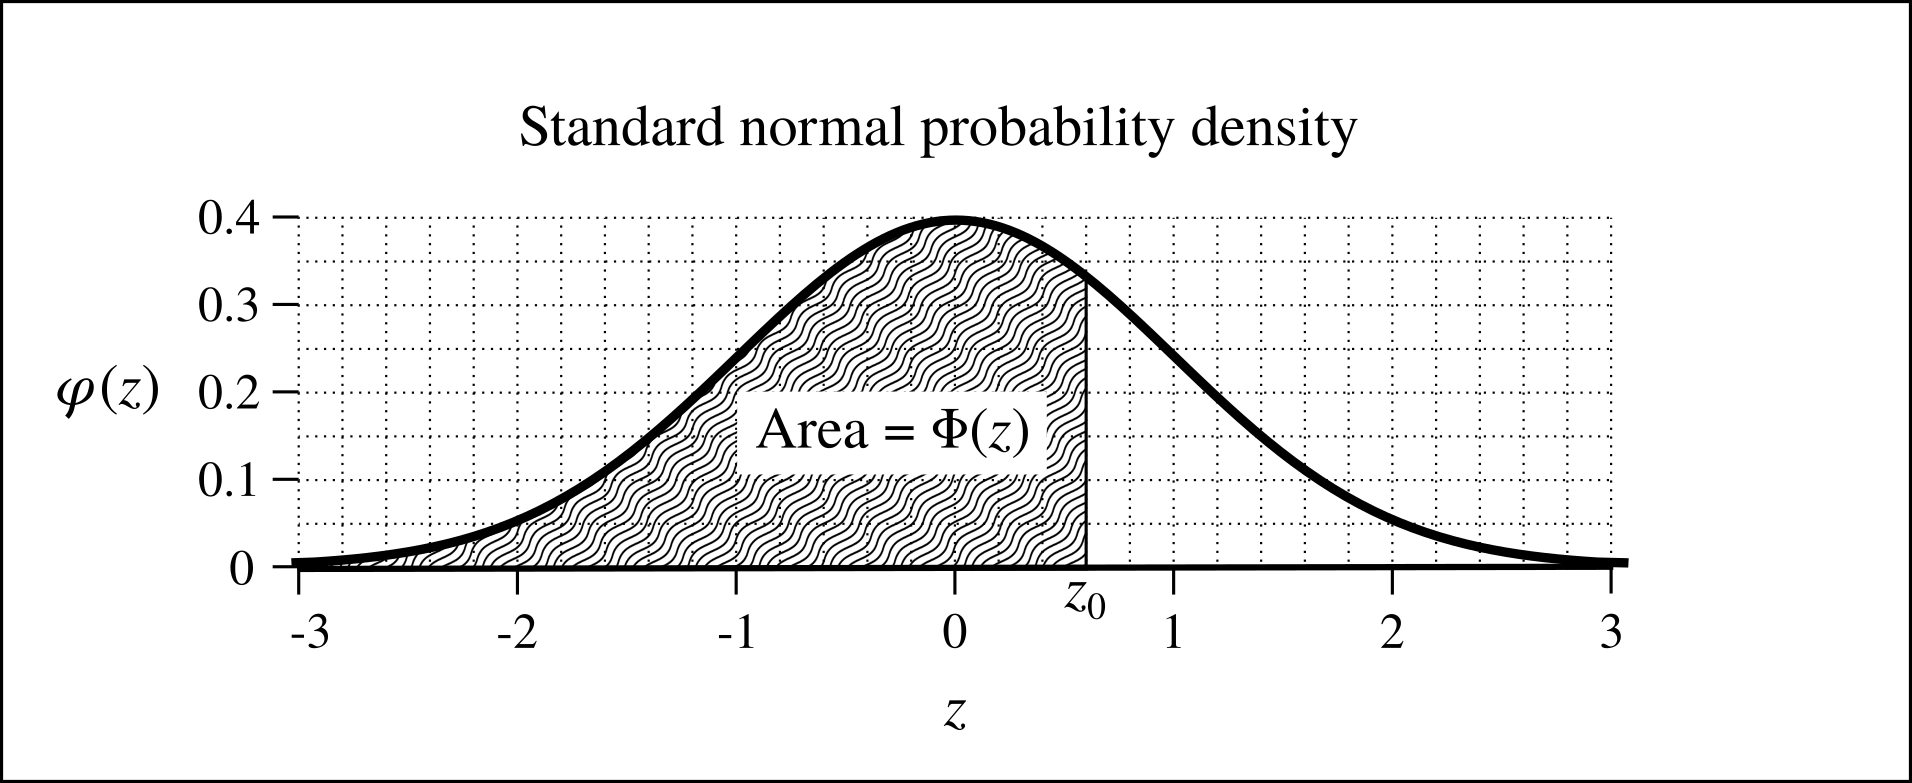
\includegraphics[scale=.7]{snpdarea.png}
\end{center}
If we repeat the process of finding the areas from $-\infty$ to any $z$, we get the cumulative distribution.
\begin{center}
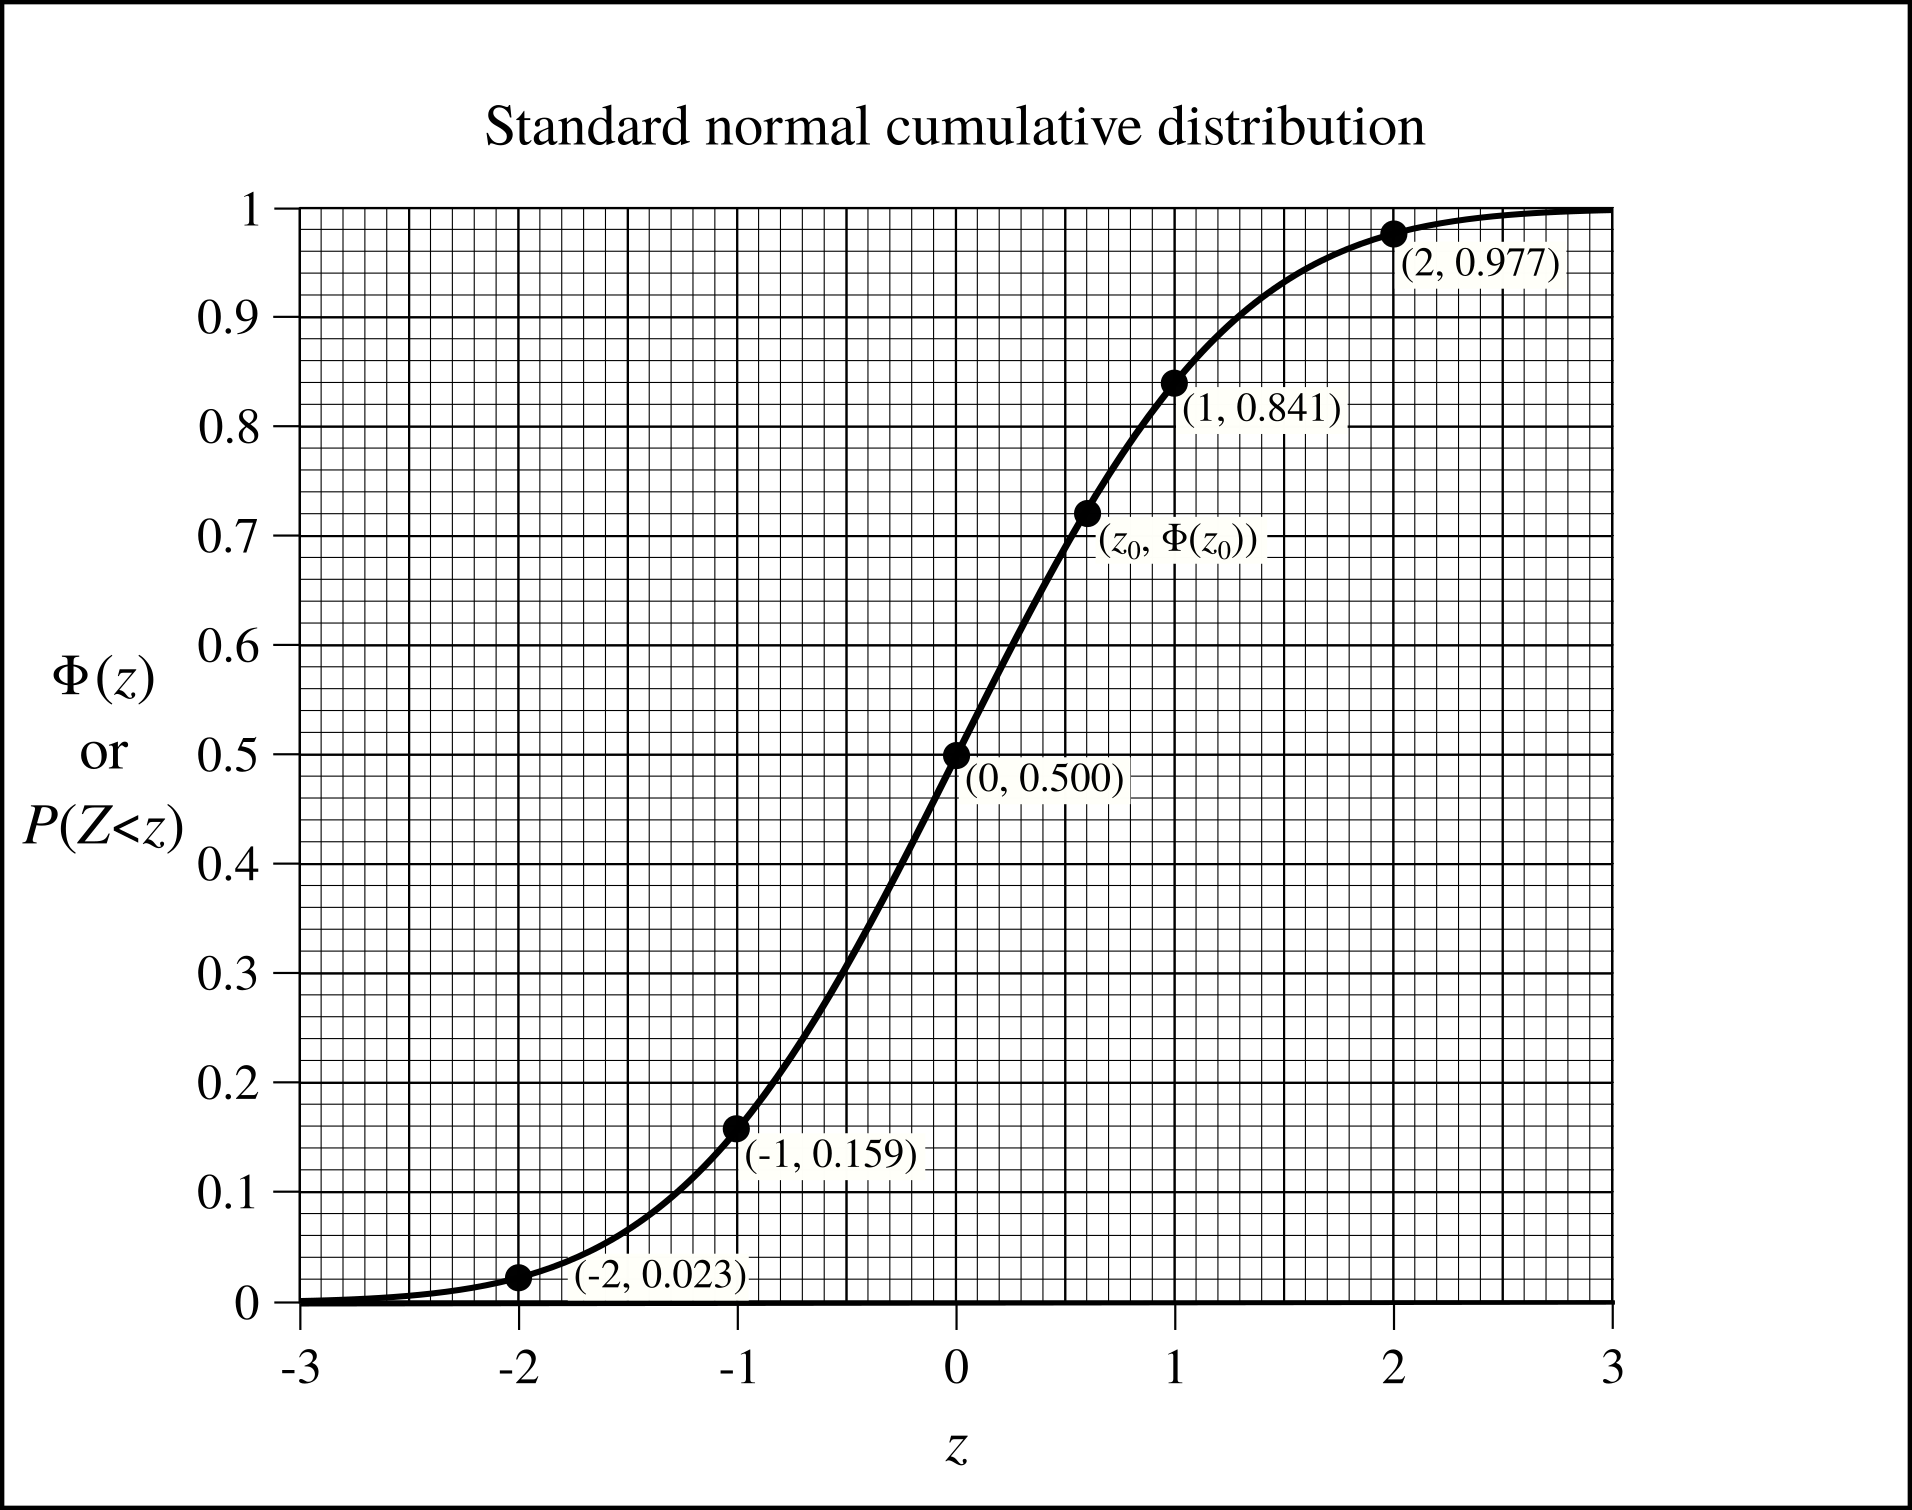
\includegraphics[scale=.7]{sncd.png}
\end{center}

Notice the notation. We use a lower-case phi, $\varphi$, for the density function and an upper-case phi ,$\Phi$, for the cumulative function.

The standard normal table gives precise values of $\Phi$ as a function of $z$. (See next page.)

{\tiny 
\begin{center}
\begin{multicols}{8}
\begin{tabular}{|c|c|}\hline
$z$ & $\Phi(z)$ \\ \hline
-3.00 & 0.0013\\
-2.99 & 0.0014\\
-2.98 & 0.0014\\
-2.97 & 0.0015\\
-2.96 & 0.0015\\
-2.95 & 0.0016\\
-2.94 & 0.0016\\
-2.93 & 0.0017\\
-2.92 & 0.0018\\
-2.91 & 0.0018\\
-2.90 & 0.0019\\
-2.89 & 0.0019\\
-2.88 & 0.0020\\
-2.87 & 0.0021\\
-2.86 & 0.0021\\
-2.85 & 0.0022\\
-2.84 & 0.0023\\
-2.83 & 0.0023\\
-2.82 & 0.0024\\
-2.81 & 0.0025\\
-2.80 & 0.0026\\
-2.79 & 0.0026\\
-2.78 & 0.0027\\
-2.77 & 0.0028\\
-2.76 & 0.0029\\
-2.75 & 0.0030\\
-2.74 & 0.0031\\
-2.73 & 0.0032\\
-2.72 & 0.0033\\
-2.71 & 0.0034\\
-2.70 & 0.0035\\
-2.69 & 0.0036\\
-2.68 & 0.0037\\
-2.67 & 0.0038\\
-2.66 & 0.0039\\
-2.65 & 0.0040\\
-2.64 & 0.0041\\
-2.63 & 0.0043\\
-2.62 & 0.0044\\
-2.61 & 0.0045\\
-2.60 & 0.0047\\
-2.59 & 0.0048\\
-2.58 & 0.0049\\
-2.57 & 0.0051\\
-2.56 & 0.0052\\
-2.55 & 0.0054\\
-2.54 & 0.0055\\
-2.53 & 0.0057\\
-2.52 & 0.0059\\
-2.51 & 0.0060\\
-2.50 & 0.0062\\
-2.49 & 0.0064\\
-2.48 & 0.0066\\
-2.47 & 0.0068\\
-2.46 & 0.0069\\
-2.45 & 0.0071\\
-2.44 & 0.0073\\
-2.43 & 0.0075\\
-2.42 & 0.0078\\
-2.41 & 0.0080\\
-2.40 & 0.0082\\
-2.39 & 0.0084\\
-2.38 & 0.0087\\
-2.37 & 0.0089\\
-2.36 & 0.0091\\
-2.35 & 0.0094\\
-2.34 & 0.0096\\
-2.33 & 0.0099\\
-2.32 & 0.0102\\
-2.31 & 0.0104\\
-2.30 & 0.0107\\
-2.29 & 0.0110\\
-2.28 & 0.0113\\
-2.27 & 0.0116\\
-2.26 & 0.0119\\
-2.25 & 0.0122\\
-2.24 & 0.0125\\
-2.23 & 0.0129\\
-2.22 & 0.0132\\
-2.21 & 0.0136\\
-2.20 & 0.0139\\
-2.19 & 0.0143\\
-2.18 & 0.0146\\
-2.17 & 0.0150\\
-2.16 & 0.0154\\
-2.15 & 0.0158\\
-2.14 & 0.0162\\
-2.13 & 0.0166\\
-2.12 & 0.0170\\
-2.11 & 0.0174\\
-2.10 & 0.0179\\
-2.09 & 0.0183\\
-2.08 & 0.0188\\
-2.07 & 0.0192\\
-2.06 & 0.0197\\
-2.05 & 0.0202\\
-2.04 & 0.0207\\
-2.03 & 0.0212\\
-2.02 & 0.0217\\
-2.01 & 0.0222\\
-2.00 & 0.0228\\
\hline \end{tabular}

\begin{tabular}{|c|c|}\hline
$z$ & $\Phi(z)$ \\ \hline
-2.00 & 0.0228\\
-1.99 & 0.0233\\
-1.98 & 0.0239\\
-1.97 & 0.0244\\
-1.96 & 0.0250\\
-1.95 & 0.0256\\
-1.94 & 0.0262\\
-1.93 & 0.0268\\
-1.92 & 0.0274\\
-1.91 & 0.0281\\
-1.90 & 0.0287\\
-1.89 & 0.0294\\
-1.88 & 0.0301\\
-1.87 & 0.0307\\
-1.86 & 0.0314\\
-1.85 & 0.0322\\
-1.84 & 0.0329\\
-1.83 & 0.0336\\
-1.82 & 0.0344\\
-1.81 & 0.0351\\
-1.80 & 0.0359\\
-1.79 & 0.0367\\
-1.78 & 0.0375\\
-1.77 & 0.0384\\
-1.76 & 0.0392\\
-1.75 & 0.0401\\
-1.74 & 0.0409\\
-1.73 & 0.0418\\
-1.72 & 0.0427\\
-1.71 & 0.0436\\
-1.70 & 0.0446\\
-1.69 & 0.0455\\
-1.68 & 0.0465\\
-1.67 & 0.0475\\
-1.66 & 0.0485\\
-1.65 & 0.0495\\
-1.64 & 0.0505\\
-1.63 & 0.0516\\
-1.62 & 0.0526\\
-1.61 & 0.0537\\
-1.60 & 0.0548\\
-1.59 & 0.0559\\
-1.58 & 0.0571\\
-1.57 & 0.0582\\
-1.56 & 0.0594\\
-1.55 & 0.0606\\
-1.54 & 0.0618\\
-1.53 & 0.0630\\
-1.52 & 0.0643\\
-1.51 & 0.0655\\
-1.50 & 0.0668\\
-1.49 & 0.0681\\
-1.48 & 0.0694\\
-1.47 & 0.0708\\
-1.46 & 0.0721\\
-1.45 & 0.0735\\
-1.44 & 0.0749\\
-1.43 & 0.0764\\
-1.42 & 0.0778\\
-1.41 & 0.0793\\
-1.40 & 0.0808\\
-1.39 & 0.0823\\
-1.38 & 0.0838\\
-1.37 & 0.0853\\
-1.36 & 0.0869\\
-1.35 & 0.0885\\
-1.34 & 0.0901\\
-1.33 & 0.0918\\
-1.32 & 0.0934\\
-1.31 & 0.0951\\
-1.30 & 0.0968\\
-1.29 & 0.0985\\
-1.28 & 0.1003\\
-1.27 & 0.1020\\
-1.26 & 0.1038\\
-1.25 & 0.1056\\
-1.24 & 0.1075\\
-1.23 & 0.1093\\
-1.22 & 0.1112\\
-1.21 & 0.1131\\
-1.20 & 0.1151\\
-1.19 & 0.1170\\
-1.18 & 0.1190\\
-1.17 & 0.1210\\
-1.16 & 0.1230\\
-1.15 & 0.1251\\
-1.14 & 0.1271\\
-1.13 & 0.1292\\
-1.12 & 0.1314\\
-1.11 & 0.1335\\
-1.10 & 0.1357\\
-1.09 & 0.1379\\
-1.08 & 0.1401\\
-1.07 & 0.1423\\
-1.06 & 0.1446\\
-1.05 & 0.1469\\
-1.04 & 0.1492\\
-1.03 & 0.1515\\
-1.02 & 0.1539\\
-1.01 & 0.1562\\
-1.00 & 0.1587\\
\hline \end{tabular}

\begin{tabular}{|c|c|}\hline
$z$ & $\Phi(z)$ \\ \hline
-1.00 & 0.1587\\
-0.99 & 0.1611\\
-0.98 & 0.1635\\
-0.97 & 0.1660\\
-0.96 & 0.1685\\
-0.95 & 0.1711\\
-0.94 & 0.1736\\
-0.93 & 0.1762\\
-0.92 & 0.1788\\
-0.91 & 0.1814\\
-0.90 & 0.1841\\
-0.89 & 0.1867\\
-0.88 & 0.1894\\
-0.87 & 0.1922\\
-0.86 & 0.1949\\
-0.85 & 0.1977\\
-0.84 & 0.2005\\
-0.83 & 0.2033\\
-0.82 & 0.2061\\
-0.81 & 0.2090\\
-0.80 & 0.2119\\
-0.79 & 0.2148\\
-0.78 & 0.2177\\
-0.77 & 0.2206\\
-0.76 & 0.2236\\
-0.75 & 0.2266\\
-0.74 & 0.2296\\
-0.73 & 0.2327\\
-0.72 & 0.2358\\
-0.71 & 0.2389\\
-0.70 & 0.2420\\
-0.69 & 0.2451\\
-0.68 & 0.2483\\
-0.67 & 0.2514\\
-0.66 & 0.2546\\
-0.65 & 0.2578\\
-0.64 & 0.2611\\
-0.63 & 0.2643\\
-0.62 & 0.2676\\
-0.61 & 0.2709\\
-0.60 & 0.2743\\
-0.59 & 0.2776\\
-0.58 & 0.2810\\
-0.57 & 0.2843\\
-0.56 & 0.2877\\
-0.55 & 0.2912\\
-0.54 & 0.2946\\
-0.53 & 0.2981\\
-0.52 & 0.3015\\
-0.51 & 0.3050\\
-0.50 & 0.3085\\
-0.49 & 0.3121\\
-0.48 & 0.3156\\
-0.47 & 0.3192\\
-0.46 & 0.3228\\
-0.45 & 0.3264\\
-0.44 & 0.3300\\
-0.43 & 0.3336\\
-0.42 & 0.3372\\
-0.41 & 0.3409\\
-0.40 & 0.3446\\
-0.39 & 0.3483\\
-0.38 & 0.3520\\
-0.37 & 0.3557\\
-0.36 & 0.3594\\
-0.35 & 0.3632\\
-0.34 & 0.3669\\
-0.33 & 0.3707\\
-0.32 & 0.3745\\
-0.31 & 0.3783\\
-0.30 & 0.3821\\
-0.29 & 0.3859\\
-0.28 & 0.3897\\
-0.27 & 0.3936\\
-0.26 & 0.3974\\
-0.25 & 0.4013\\
-0.24 & 0.4052\\
-0.23 & 0.4090\\
-0.22 & 0.4129\\
-0.21 & 0.4168\\
-0.20 & 0.4207\\
-0.19 & 0.4247\\
-0.18 & 0.4286\\
-0.17 & 0.4325\\
-0.16 & 0.4364\\
-0.15 & 0.4404\\
-0.14 & 0.4443\\
-0.13 & 0.4483\\
-0.12 & 0.4522\\
-0.11 & 0.4562\\
-0.10 & 0.4602\\
-0.09 & 0.4641\\
-0.08 & 0.4681\\
-0.07 & 0.4721\\
-0.06 & 0.4761\\
-0.05 & 0.4801\\
-0.04 & 0.4840\\
-0.03 & 0.4880\\
-0.02 & 0.4920\\
-0.01 & 0.4960\\
0.00 & 0.5000\\
\hline \end{tabular}

\begin{tabular}{|c|c|}\hline
$z$ & $\Phi(z)$ \\ \hline
0.00 & 0.5000\\
0.01 & 0.5040\\
0.02 & 0.5080\\
0.03 & 0.5120\\
0.04 & 0.5160\\
0.05 & 0.5199\\
0.06 & 0.5239\\
0.07 & 0.5279\\
0.08 & 0.5319\\
0.09 & 0.5359\\
0.10 & 0.5398\\
0.11 & 0.5438\\
0.12 & 0.5478\\
0.13 & 0.5517\\
0.14 & 0.5557\\
0.15 & 0.5596\\
0.16 & 0.5636\\
0.17 & 0.5675\\
0.18 & 0.5714\\
0.19 & 0.5753\\
0.20 & 0.5793\\
0.21 & 0.5832\\
0.22 & 0.5871\\
0.23 & 0.5910\\
0.24 & 0.5948\\
0.25 & 0.5987\\
0.26 & 0.6026\\
0.27 & 0.6064\\
0.28 & 0.6103\\
0.29 & 0.6141\\
0.30 & 0.6179\\
0.31 & 0.6217\\
0.32 & 0.6255\\
0.33 & 0.6293\\
0.34 & 0.6331\\
0.35 & 0.6368\\
0.36 & 0.6406\\
0.37 & 0.6443\\
0.38 & 0.6480\\
0.39 & 0.6517\\
0.40 & 0.6554\\
0.41 & 0.6591\\
0.42 & 0.6628\\
0.43 & 0.6664\\
0.44 & 0.6700\\
0.45 & 0.6736\\
0.46 & 0.6772\\
0.47 & 0.6808\\
0.48 & 0.6844\\
0.49 & 0.6879\\
0.50 & 0.6915\\
0.51 & 0.6950\\
0.52 & 0.6985\\
0.53 & 0.7019\\
0.54 & 0.7054\\
0.55 & 0.7088\\
0.56 & 0.7123\\
0.57 & 0.7157\\
0.58 & 0.7190\\
0.59 & 0.7224\\
0.60 & 0.7257\\
0.61 & 0.7291\\
0.62 & 0.7324\\
0.63 & 0.7357\\
0.64 & 0.7389\\
0.65 & 0.7422\\
0.66 & 0.7454\\
0.67 & 0.7486\\
0.68 & 0.7517\\
0.69 & 0.7549\\
0.70 & 0.7580\\
0.71 & 0.7611\\
0.72 & 0.7642\\
0.73 & 0.7673\\
0.74 & 0.7704\\
0.75 & 0.7734\\
0.76 & 0.7764\\
0.77 & 0.7794\\
0.78 & 0.7823\\
0.79 & 0.7852\\
0.80 & 0.7881\\
0.81 & 0.7910\\
0.82 & 0.7939\\
0.83 & 0.7967\\
0.84 & 0.7995\\
0.85 & 0.8023\\
0.86 & 0.8051\\
0.87 & 0.8078\\
0.88 & 0.8106\\
0.89 & 0.8133\\
0.90 & 0.8159\\
0.91 & 0.8186\\
0.92 & 0.8212\\
0.93 & 0.8238\\
0.94 & 0.8264\\
0.95 & 0.8289\\
0.96 & 0.8315\\
0.97 & 0.8340\\
0.98 & 0.8365\\
0.99 & 0.8389\\
1.00 & 0.8413\\
\hline \end{tabular}

\begin{tabular}{|c|c|}\hline
$z$ & $\Phi(z)$ \\ \hline
1.00 & 0.8413\\
1.01 & 0.8438\\
1.02 & 0.8461\\
1.03 & 0.8485\\
1.04 & 0.8508\\
1.05 & 0.8531\\
1.06 & 0.8554\\
1.07 & 0.8577\\
1.08 & 0.8599\\
1.09 & 0.8621\\
1.10 & 0.8643\\
1.11 & 0.8665\\
1.12 & 0.8686\\
1.13 & 0.8708\\
1.14 & 0.8729\\
1.15 & 0.8749\\
1.16 & 0.8770\\
1.17 & 0.8790\\
1.18 & 0.8810\\
1.19 & 0.8830\\
1.20 & 0.8849\\
1.21 & 0.8869\\
1.22 & 0.8888\\
1.23 & 0.8907\\
1.24 & 0.8925\\
1.25 & 0.8944\\
1.26 & 0.8962\\
1.27 & 0.8980\\
1.28 & 0.8997\\
1.29 & 0.9015\\
1.30 & 0.9032\\
1.31 & 0.9049\\
1.32 & 0.9066\\
1.33 & 0.9082\\
1.34 & 0.9099\\
1.35 & 0.9115\\
1.36 & 0.9131\\
1.37 & 0.9147\\
1.38 & 0.9162\\
1.39 & 0.9177\\
1.40 & 0.9192\\
1.41 & 0.9207\\
1.42 & 0.9222\\
1.43 & 0.9236\\
1.44 & 0.9251\\
1.45 & 0.9265\\
1.46 & 0.9279\\
1.47 & 0.9292\\
1.48 & 0.9306\\
1.49 & 0.9319\\
1.50 & 0.9332\\
1.51 & 0.9345\\
1.52 & 0.9357\\
1.53 & 0.9370\\
1.54 & 0.9382\\
1.55 & 0.9394\\
1.56 & 0.9406\\
1.57 & 0.9418\\
1.58 & 0.9429\\
1.59 & 0.9441\\
1.60 & 0.9452\\
1.61 & 0.9463\\
1.62 & 0.9474\\
1.63 & 0.9484\\
1.64 & 0.9495\\
1.65 & 0.9505\\
1.66 & 0.9515\\
1.67 & 0.9525\\
1.68 & 0.9535\\
1.69 & 0.9545\\
1.70 & 0.9554\\
1.71 & 0.9564\\
1.72 & 0.9573\\
1.73 & 0.9582\\
1.74 & 0.9591\\
1.75 & 0.9599\\
1.76 & 0.9608\\
1.77 & 0.9616\\
1.78 & 0.9625\\
1.79 & 0.9633\\
1.80 & 0.9641\\
1.81 & 0.9649\\
1.82 & 0.9656\\
1.83 & 0.9664\\
1.84 & 0.9671\\
1.85 & 0.9678\\
1.86 & 0.9686\\
1.87 & 0.9693\\
1.88 & 0.9699\\
1.89 & 0.9706\\
1.90 & 0.9713\\
1.91 & 0.9719\\
1.92 & 0.9726\\
1.93 & 0.9732\\
1.94 & 0.9738\\
1.95 & 0.9744\\
1.96 & 0.9750\\
1.97 & 0.9756\\
1.98 & 0.9761\\
1.99 & 0.9767\\
2.00 & 0.9772\\
\hline \end{tabular}

\begin{tabular}{|c|c|}\hline
$z$ & $\Phi(z)$ \\ \hline
2.00 & 0.9772\\
2.01 & 0.9778\\
2.02 & 0.9783\\
2.03 & 0.9788\\
2.04 & 0.9793\\
2.05 & 0.9798\\
2.06 & 0.9803\\
2.07 & 0.9808\\
2.08 & 0.9812\\
2.09 & 0.9817\\
2.10 & 0.9821\\
2.11 & 0.9826\\
2.12 & 0.9830\\
2.13 & 0.9834\\
2.14 & 0.9838\\
2.15 & 0.9842\\
2.16 & 0.9846\\
2.17 & 0.9850\\
2.18 & 0.9854\\
2.19 & 0.9857\\
2.20 & 0.9861\\
2.21 & 0.9864\\
2.22 & 0.9868\\
2.23 & 0.9871\\
2.24 & 0.9875\\
2.25 & 0.9878\\
2.26 & 0.9881\\
2.27 & 0.9884\\
2.28 & 0.9887\\
2.29 & 0.9890\\
2.30 & 0.9893\\
2.31 & 0.9896\\
2.32 & 0.9898\\
2.33 & 0.9901\\
2.34 & 0.9904\\
2.35 & 0.9906\\
2.36 & 0.9909\\
2.37 & 0.9911\\
2.38 & 0.9913\\
2.39 & 0.9916\\
2.40 & 0.9918\\
2.41 & 0.9920\\
2.42 & 0.9922\\
2.43 & 0.9925\\
2.44 & 0.9927\\
2.45 & 0.9929\\
2.46 & 0.9931\\
2.47 & 0.9932\\
2.48 & 0.9934\\
2.49 & 0.9936\\
2.50 & 0.9938\\
2.51 & 0.9940\\
2.52 & 0.9941\\
2.53 & 0.9943\\
2.54 & 0.9945\\
2.55 & 0.9946\\
2.56 & 0.9948\\
2.57 & 0.9949\\
2.58 & 0.9951\\
2.59 & 0.9952\\
2.60 & 0.9953\\
2.61 & 0.9955\\
2.62 & 0.9956\\
2.63 & 0.9957\\
2.64 & 0.9959\\
2.65 & 0.9960\\
2.66 & 0.9961\\
2.67 & 0.9962\\
2.68 & 0.9963\\
2.69 & 0.9964\\
2.70 & 0.9965\\
2.71 & 0.9966\\
2.72 & 0.9967\\
2.73 & 0.9968\\
2.74 & 0.9969\\
2.75 & 0.9970\\
2.76 & 0.9971\\
2.77 & 0.9972\\
2.78 & 0.9973\\
2.79 & 0.9974\\
2.80 & 0.9974\\
2.81 & 0.9975\\
2.82 & 0.9976\\
2.83 & 0.9977\\
2.84 & 0.9977\\
2.85 & 0.9978\\
2.86 & 0.9979\\
2.87 & 0.9979\\
2.88 & 0.9980\\
2.89 & 0.9981\\
2.90 & 0.9981\\
2.91 & 0.9982\\
2.92 & 0.9982\\
2.93 & 0.9983\\
2.94 & 0.9984\\
2.95 & 0.9984\\
2.96 & 0.9985\\
2.97 & 0.9985\\
2.98 & 0.9986\\
2.99 & 0.9986\\
3.00 & 0.9987\\
\hline \end{tabular}


\end{multicols}
\end{center}
}

\newpage
%\newcommand{\emptybox}{\fbox{\phantom{\cfrac{aafkfhhhhha}{s}}}}
\newcommand{\emptybox}{\fbox{\text{ }\hspace{60pt}\text{ \phantom{$\cfrac{h}{h}$} }}}
\begin{enumerate}
\item For each of the following, complete the diagram so it has a shaded region and a probability statement, like the example below.
\\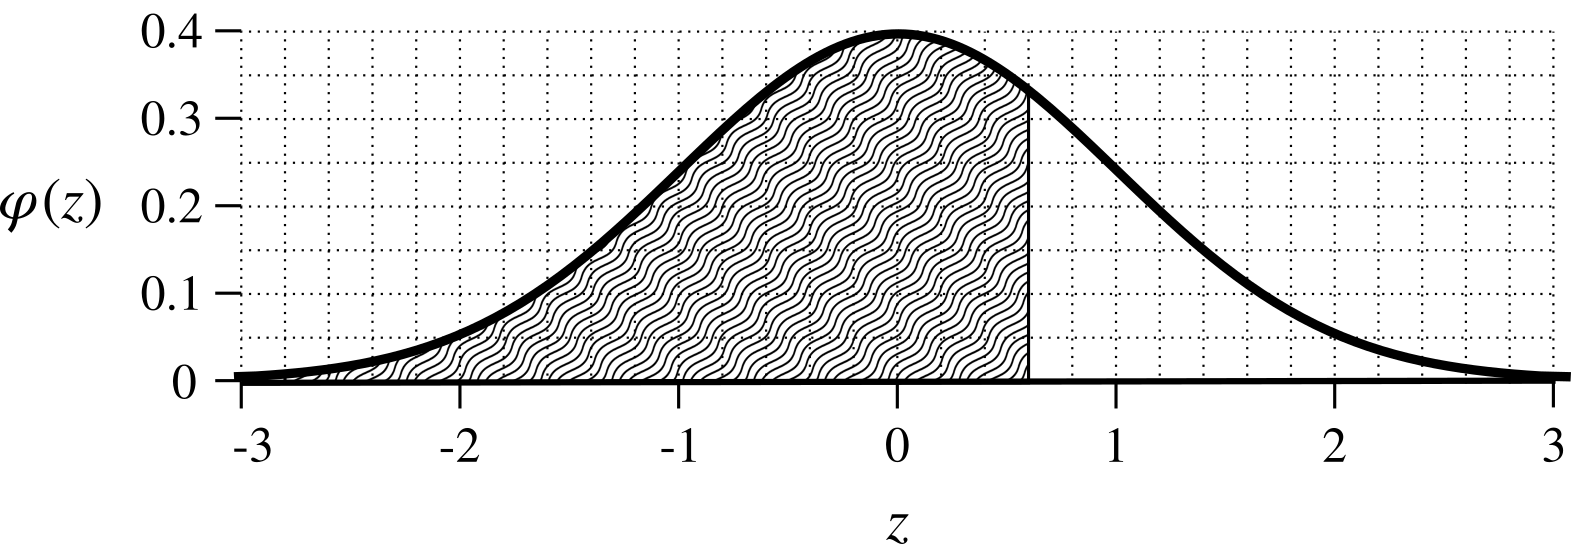
\includegraphics[scale=0.7]{0p6.png} $P(Z<0.6) = 0.7257$
\begin{enumerate}
\vfill
\item Shade the region and evaluate the probability $P(Z<-1.4)$.
\\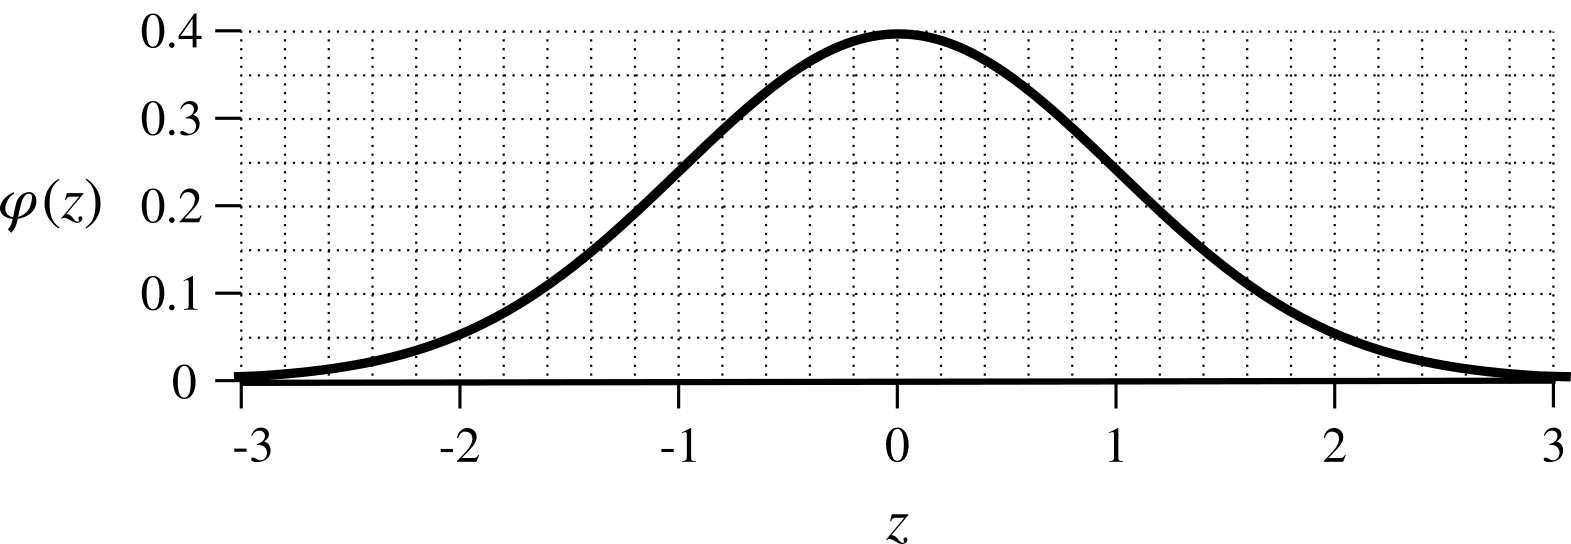
\includegraphics[scale=0.7]{blank.png} $P(Z<-1.4)=\emptybox$
\vfill
\item Shade the region and evaluate the probability $P(Z<2)$.
\\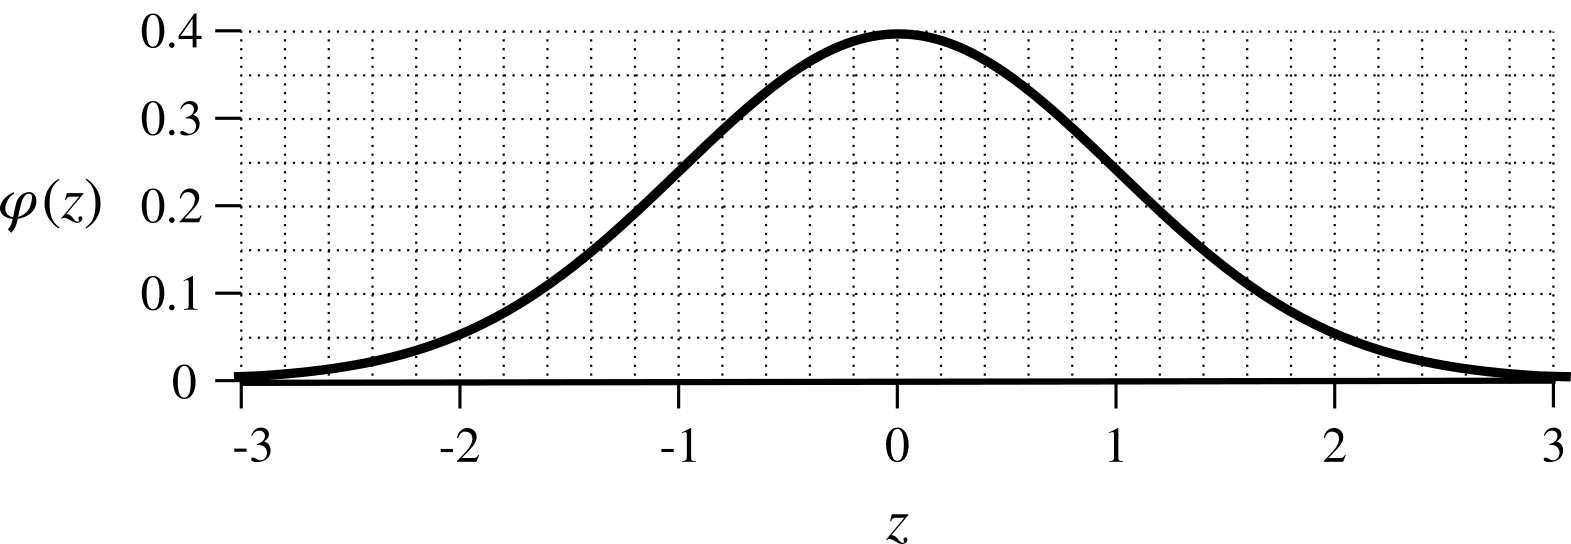
\includegraphics[scale=0.7]{blank.png} $P(Z<2)=\emptybox$
\vfill
\item From the shaded region, evaluate the probability.
\\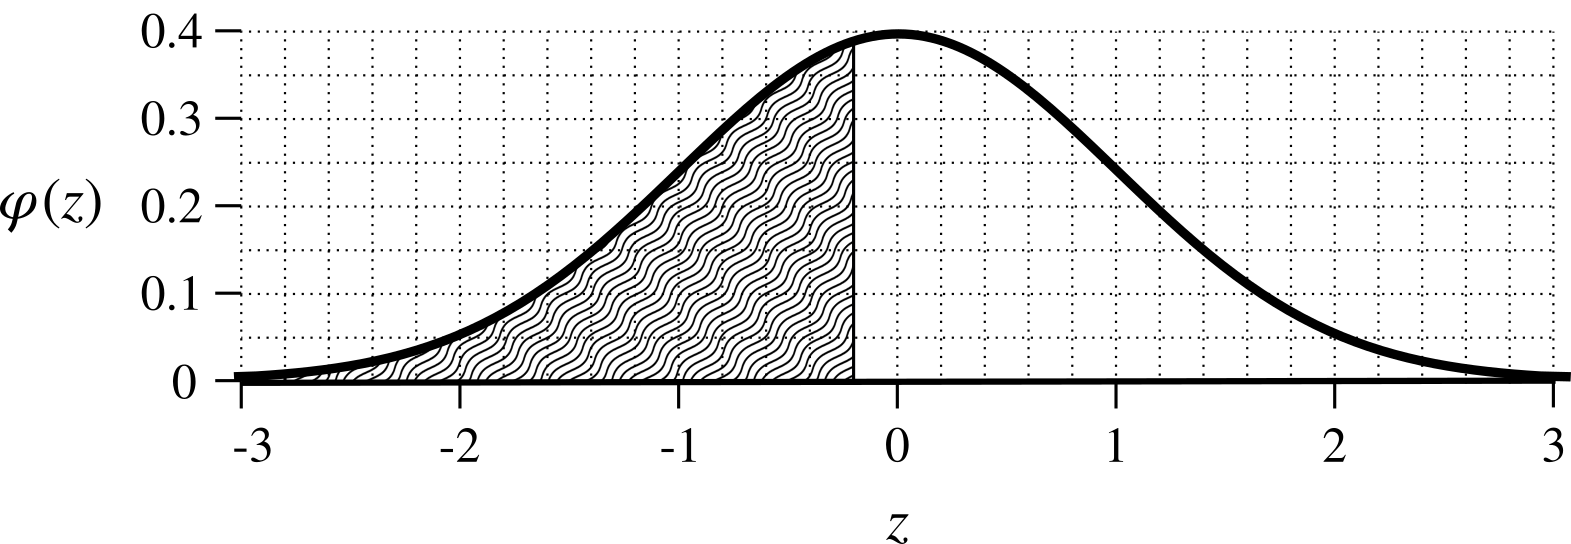
\includegraphics[scale=0.7]{n0p2.png}  $\emptybox=\emptybox$
\vfill
\end{enumerate}
\end{enumerate}

\newpage
The area under $\varphi(z)$ from $-\infty$ to $\infty$ is 1. Also, the function $\varphi(z)$ is symmetric. This leads to a useful property:
$$\Phi(-z) = 1-\Phi(z) $$
\begin{center}
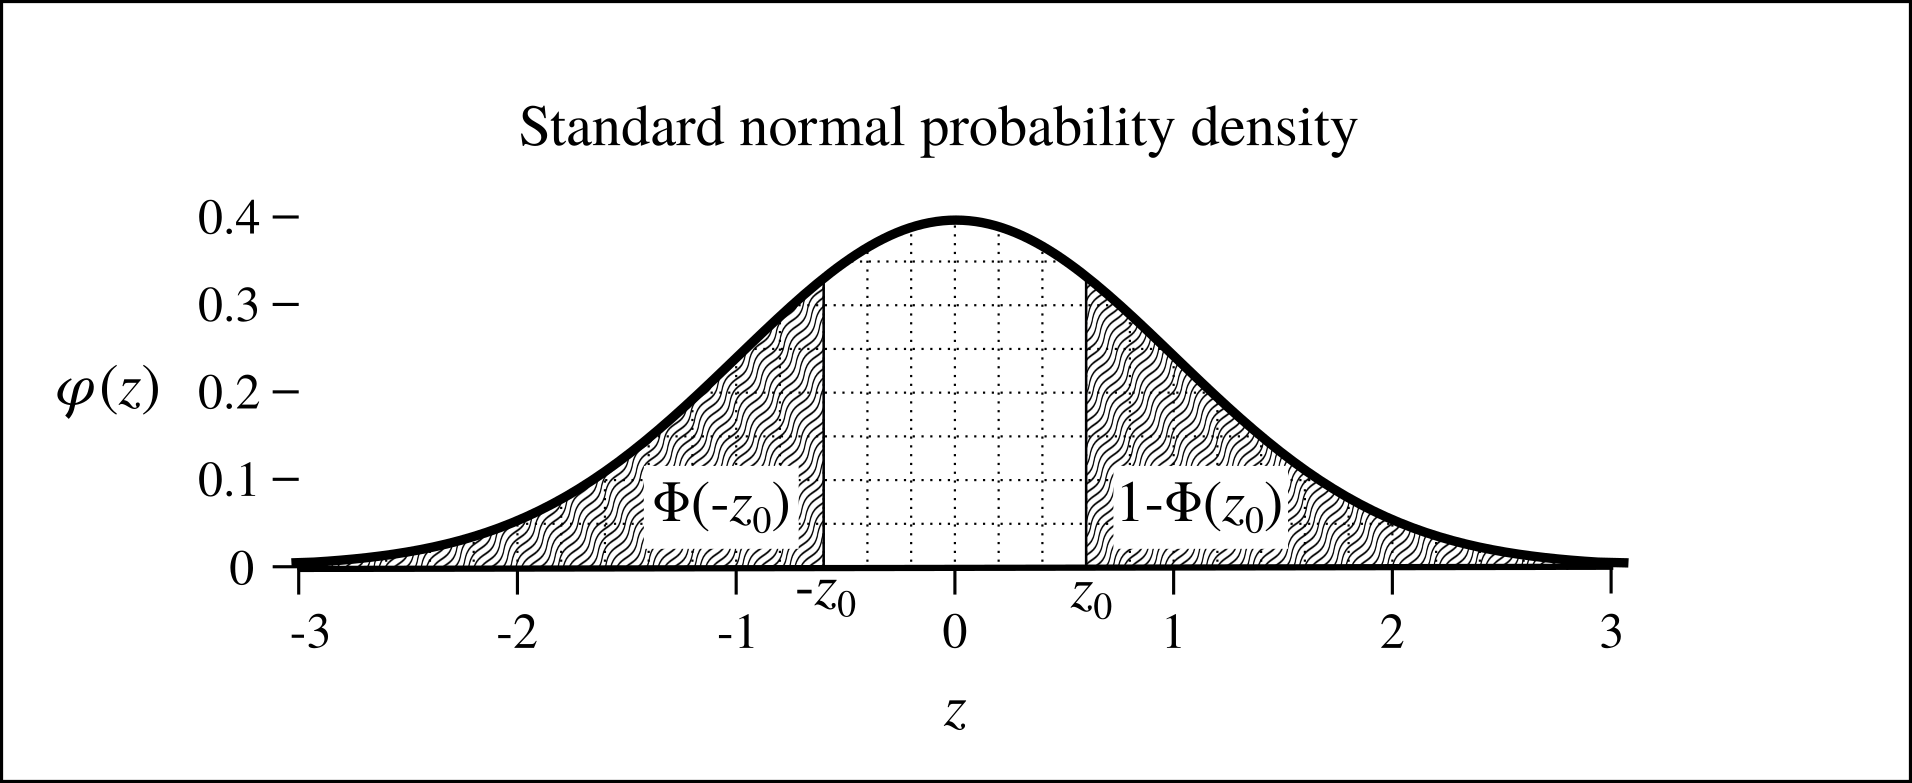
\includegraphics[scale=0.7]{prop.png}
\end{center}

There are five common areas we are asked to find: left, right, sectional, central (symmetric), and two-tailed (symmetric).
\begin{center}
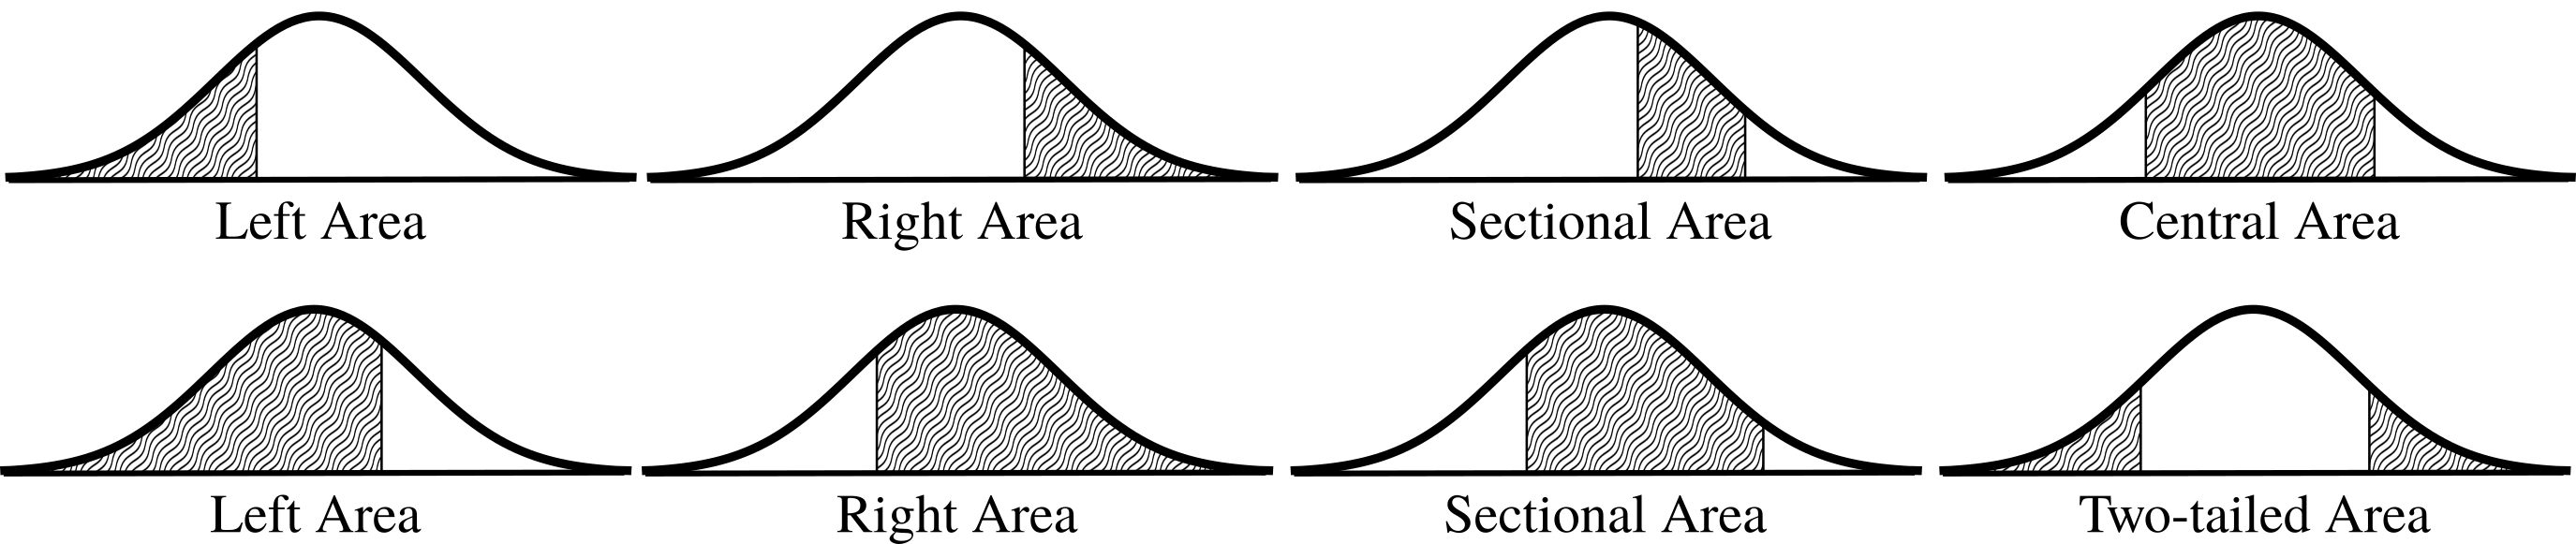
\includegraphics[scale=0.7]{types.png}
\end{center}
\begin{align*}
\texttt{Left area} &= P(Z<z)\\
 &= \Phi(z)\\\\
\texttt{Right area} &= P(Z>z) \\&= 1-\Phi(z) \\&= \Phi(-z)\\\\
\texttt{Sectional area} &= P(z_1<Z<z_2) \\&= \Phi(z_2) - \Phi(z_1)\\\\
\texttt{Central area} &= P(|Z|<z) \\&= \Phi(z)-\Phi(-z) \\&= 1-2\Phi(-z)\\ &= 2\Phi(z)-1\\\\
\texttt{Two-tailed area} &= P(|Z|>z) \\ &= 1-\Phi(z)+\Phi(-z) \\&=2-2\Phi(z) \\ &= 2\Phi(-z)
\end{align*}
\label{hi}

\newpage
\begin{enumerate}[resume]
\item For each of the following, complete the diagram so it has a shaded region and a probability statement. Also, notice that you can estimate the probability by counting the number of shaded squares; each unit square is worth 1\%.
\begin{enumerate}
\item Shade the region of and evaluate the probability that $Z$ is more than 1.6.
\\ 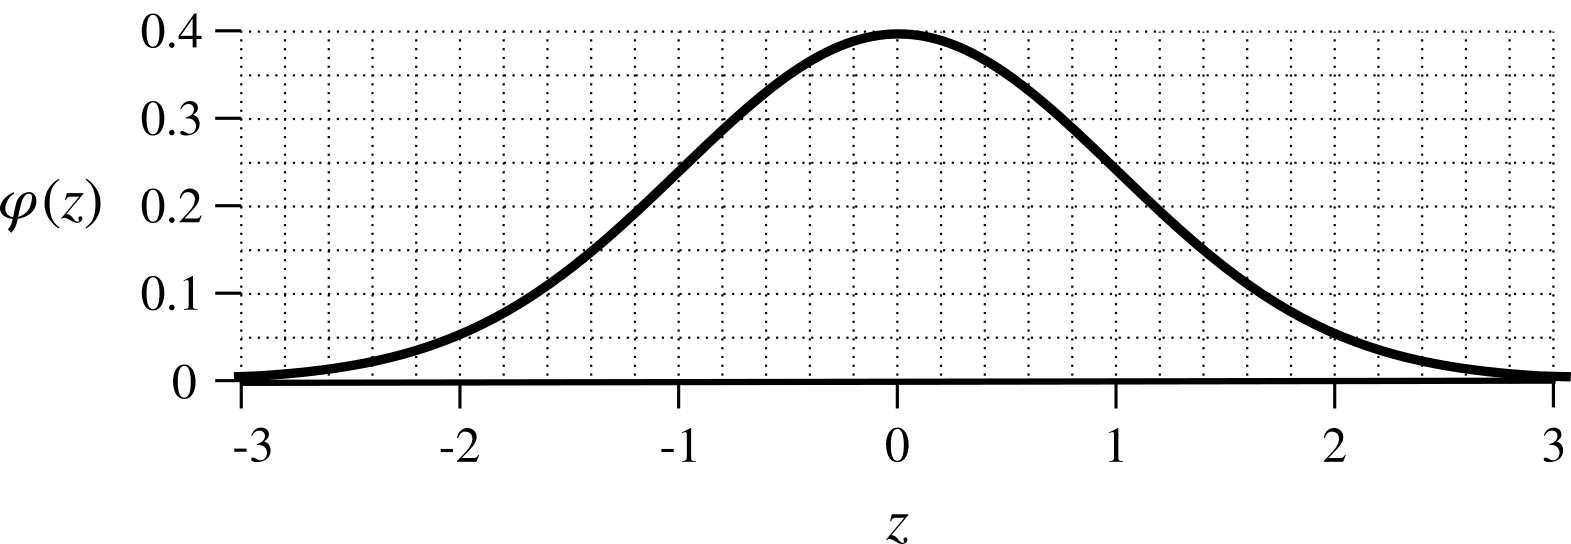
\includegraphics[scale=0.7]{blank.png}   $~~\emptybox=\emptybox$
\vfill
\item Shade the region of and evaluate the probability that $Z$ is between 0.4 and 0.6.
\\ 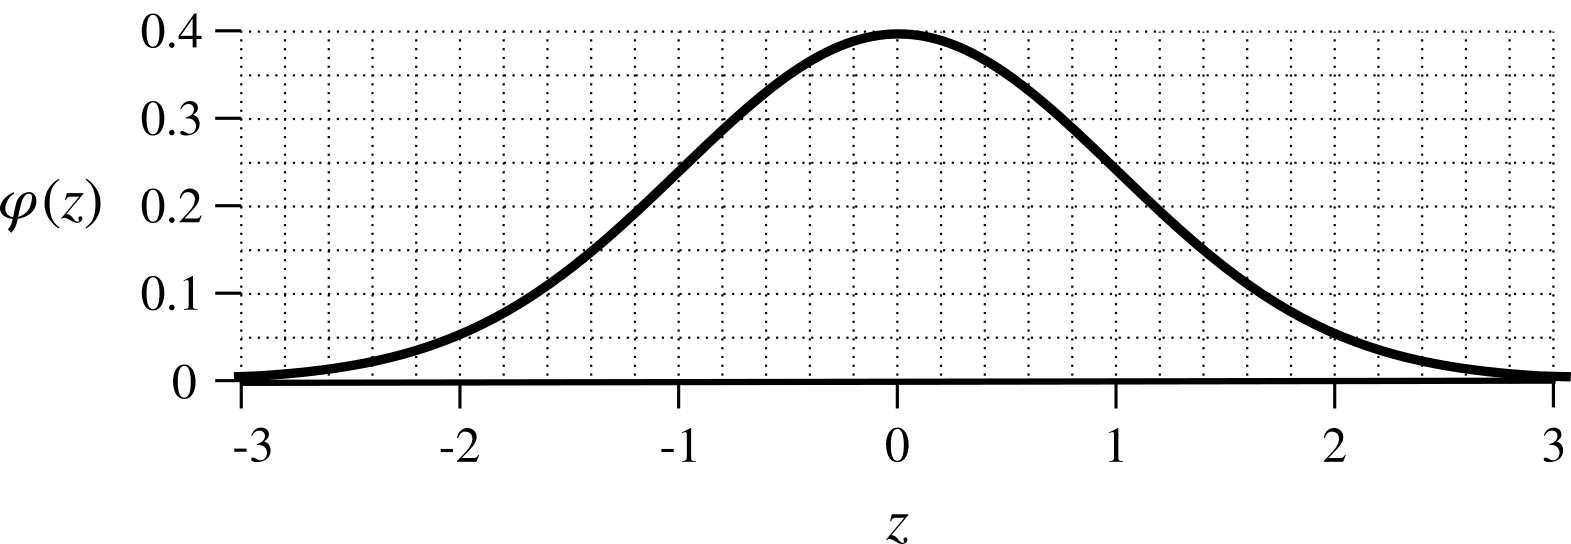
\includegraphics[scale=0.7]{blank.png}   $~~\emptybox=\emptybox$
\vfill
\item Shade the region of and evaluate the probability that $Z$ is between 1 and 2.
\\ 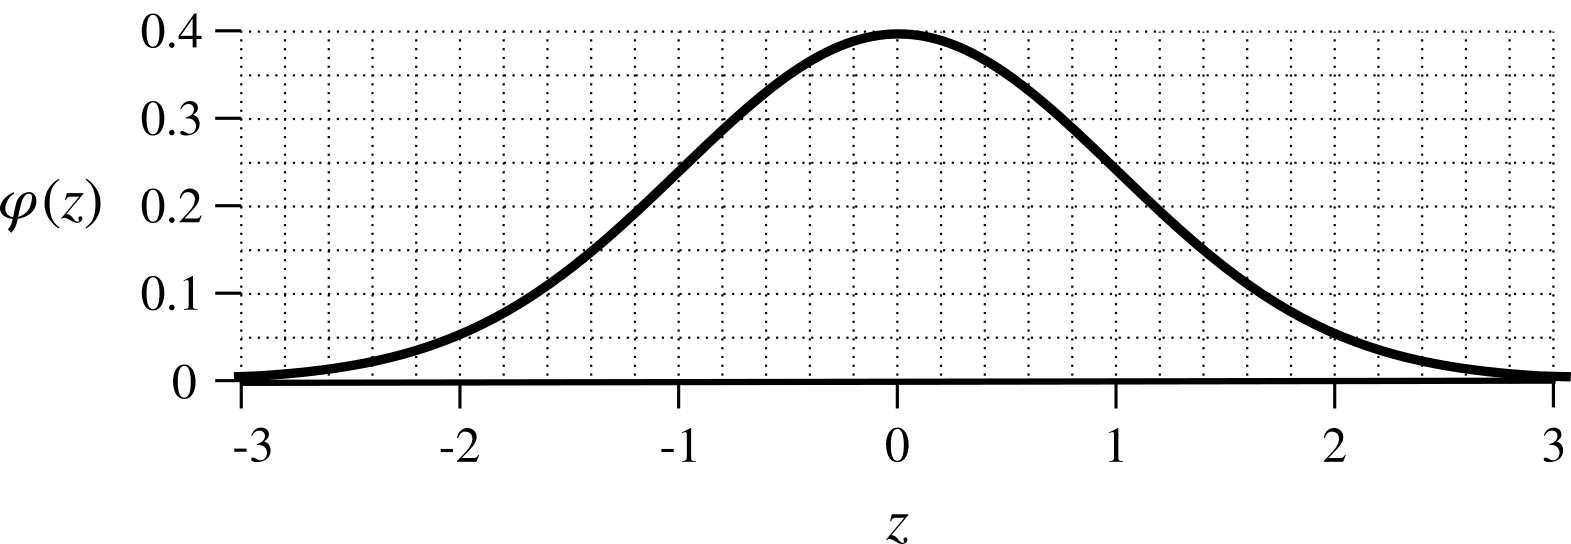
\includegraphics[scale=0.7]{blank.png}   $~~\emptybox=\emptybox$
\vfill
\item Shade the region of and evaluate the probability that $Z$ is between -0.4 and 0.4.
\\ 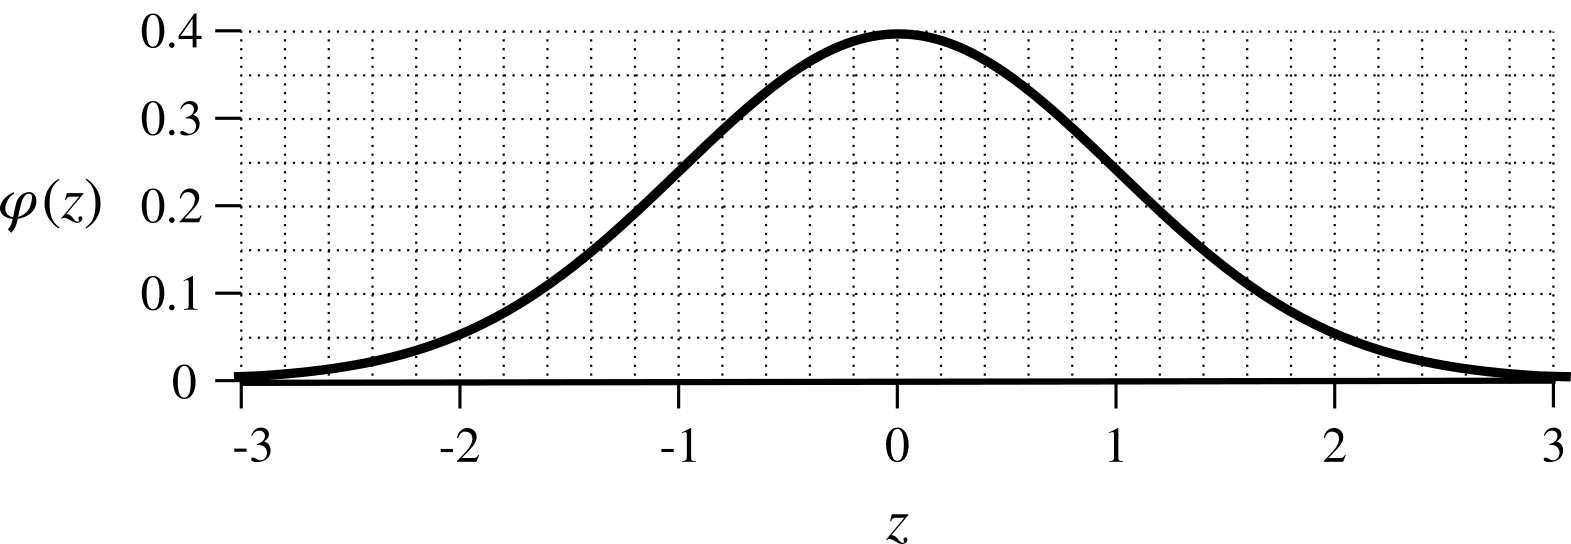
\includegraphics[scale=0.7]{blank.png}   $~~\emptybox=\emptybox$
\vfill
\item Shade the region of and evaluate the probability that $Z$ is less than -0.4 or more than 0.4.
\\ 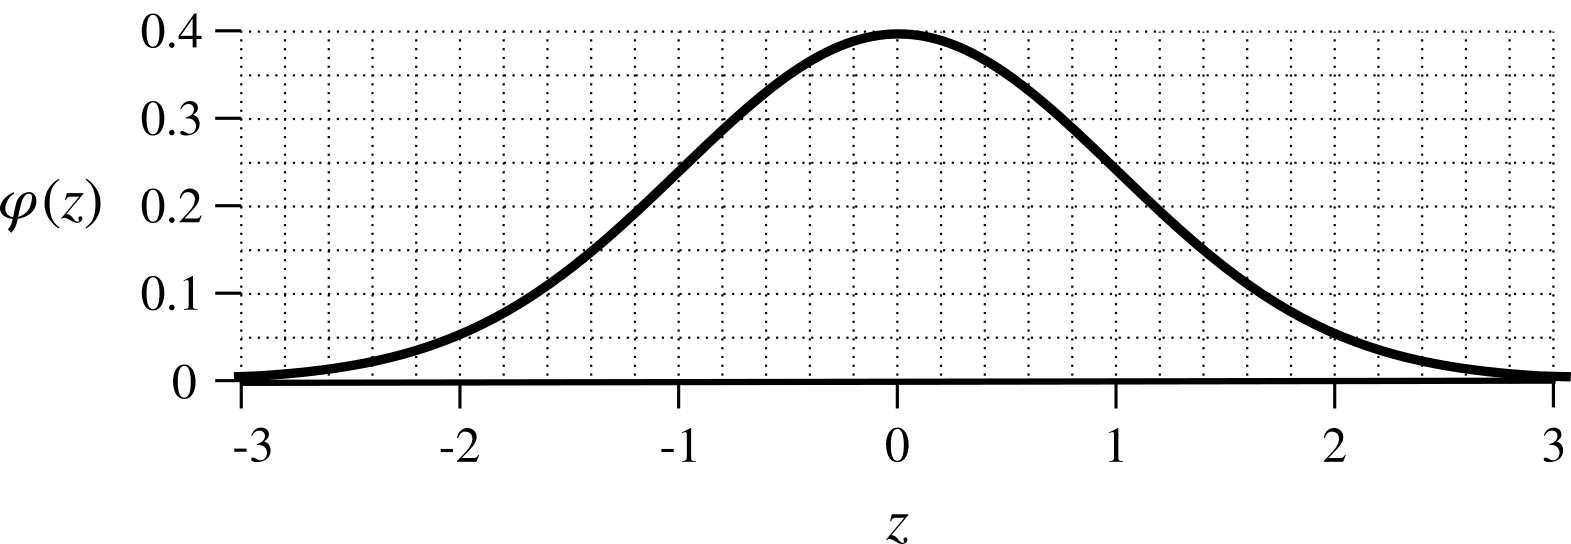
\includegraphics[scale=0.7]{blank.png}   $~~\emptybox=\emptybox$
\vfill
\end{enumerate}
\end{enumerate}



%\newpage
%\begin{enumerate}
%\item Evaluate $\Phi(1.96)$
%\vfill
%\item Evaluate $P(Z < 1.08)$
%\vfill
%\item Evaluate $P(Z > 1.08)$
%\vfill
%\item Evaluate $P(1.08 < Z < 1.96)$
%\vfill
%\item Evaluate $P(|Z| < 1.96)$, which is the same as $P(-1.96 < Z < 1.96)$
%\vfill
%\item Evaluate $P(|Z| > 1.96)$, which is the same as $P(Z < -1.96 ~~\text{OR}~~ 1.96<Z)$
%\vfill
%\end{enumerate}


\newpage
This diagram might be useful. Some of the areas seem to add imperfectly because these numbers are all rounded. Also, it should be noted that $\Phi(-3) = 0.00135 \ne 0$.\\\\
\begin{center}
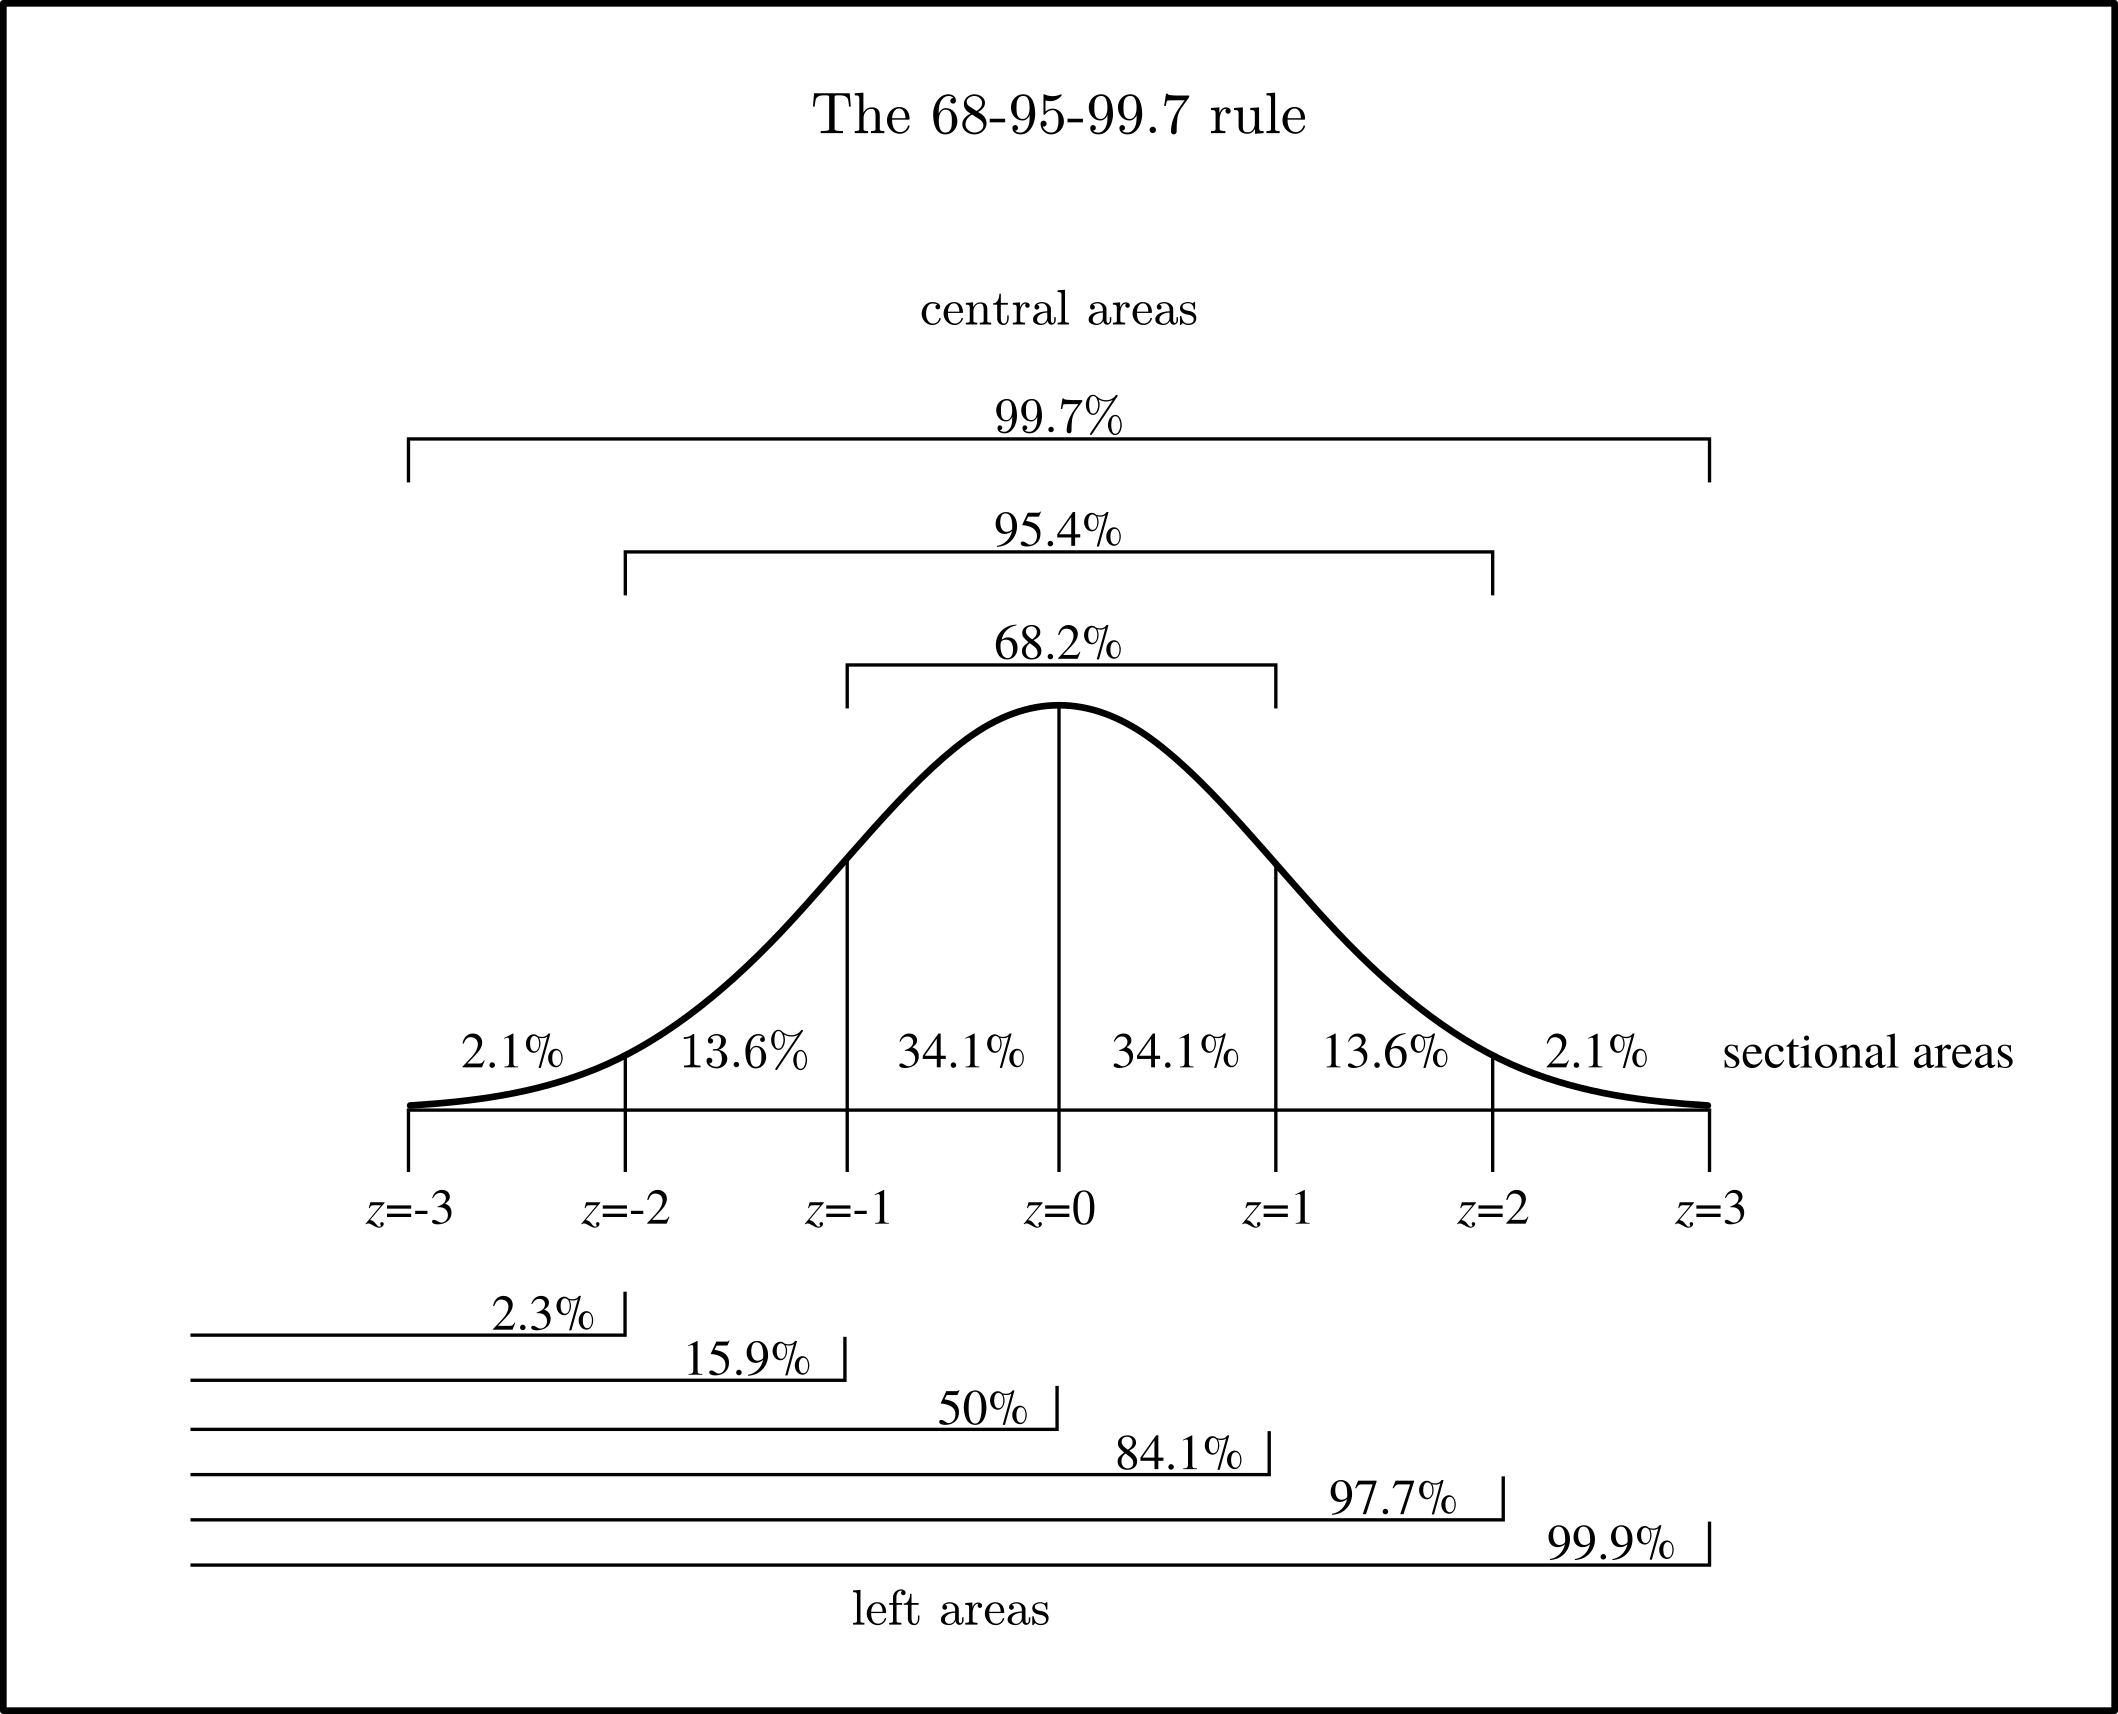
\includegraphics[scale=1]{toomuch.png}
\end{center}
\url{https://en.wikipedia.org/wiki/68-95-99.7_rule}




\newpage
\begin{enumerate}[resume]
\item By using the standard normal table (or the 68-95-99.7 rule), you should be able to determine the following probabilities. For each question, determine the probability (area) of the shaded region or regions. In cases where the bound could be $-3$ or $3$, use $-\infty$ or $\infty$ instead.  Write the answer using the ``$P(\texttt{condition}) = \texttt{number}$'' format.

\begin{enumerate}[itemsep=50pt]
\begin{multicols}{2}
\item \adjustbox{valign=t}{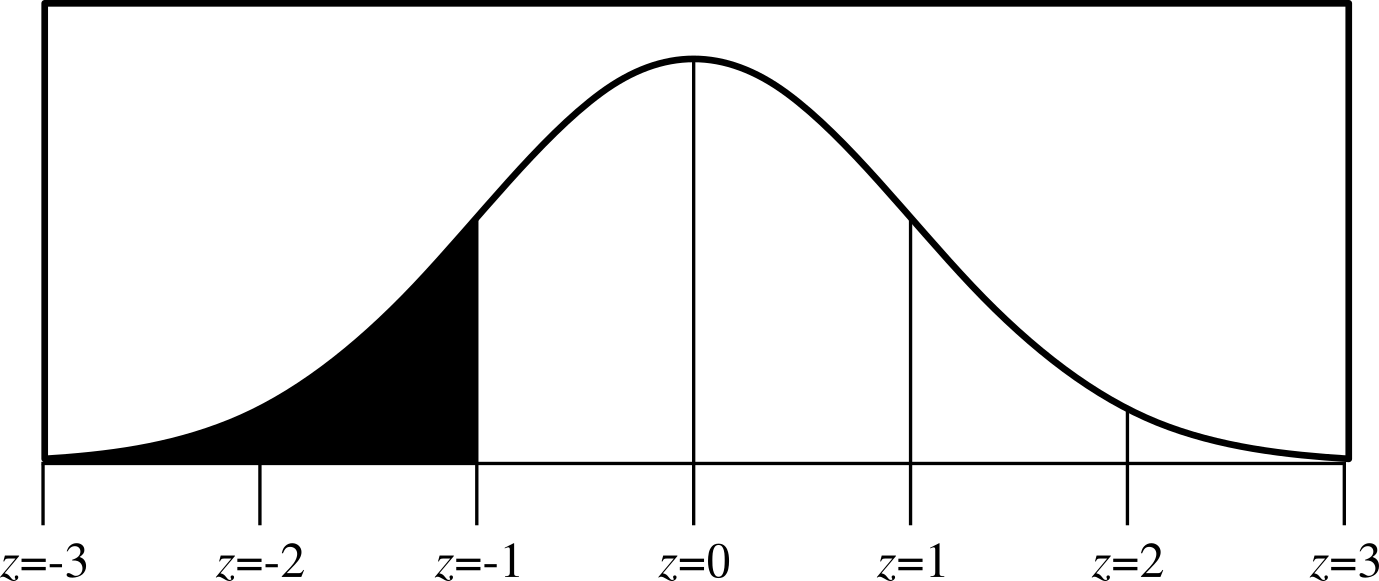
\includegraphics[scale=.5]{n3_n1.png}}
\item \adjustbox{valign=t}{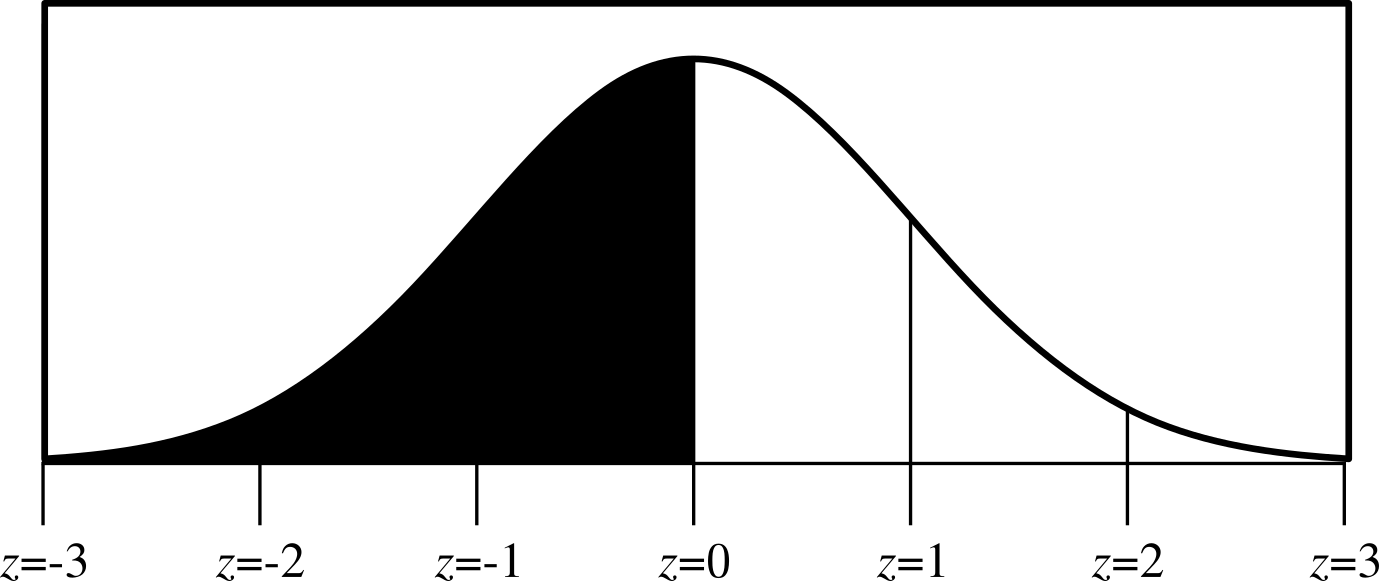
\includegraphics[scale=.5]{n3_0.png}}
\item \adjustbox{valign=t}{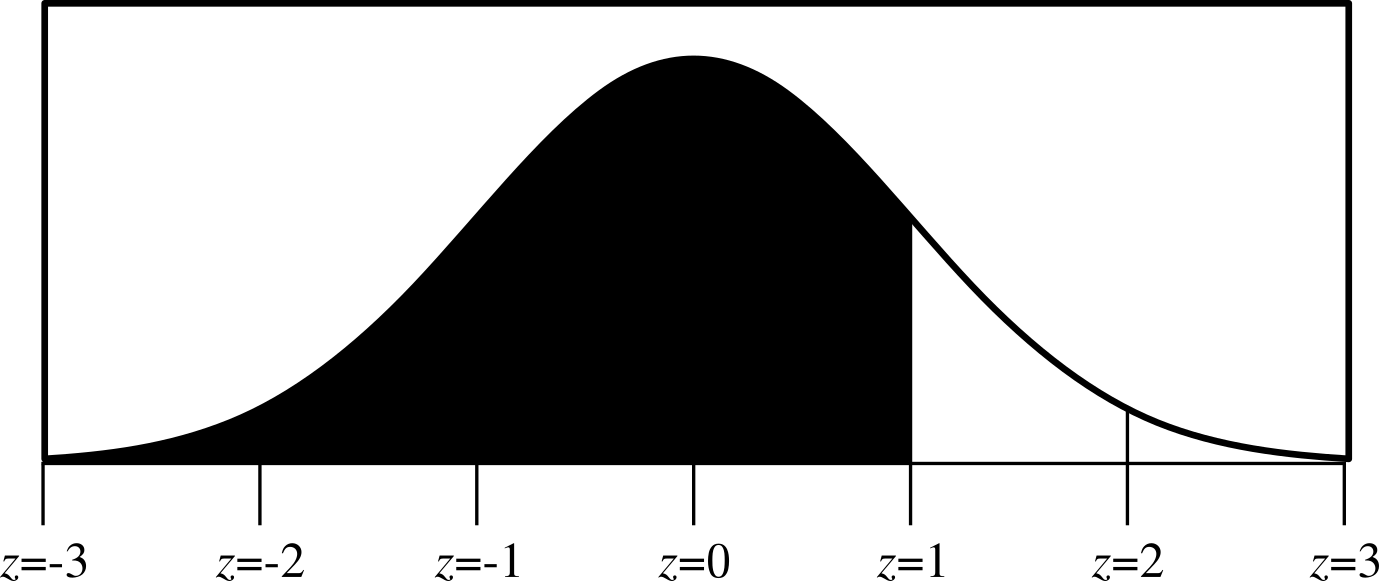
\includegraphics[scale=.5]{n3_1.png}}
\item \adjustbox{valign=t}{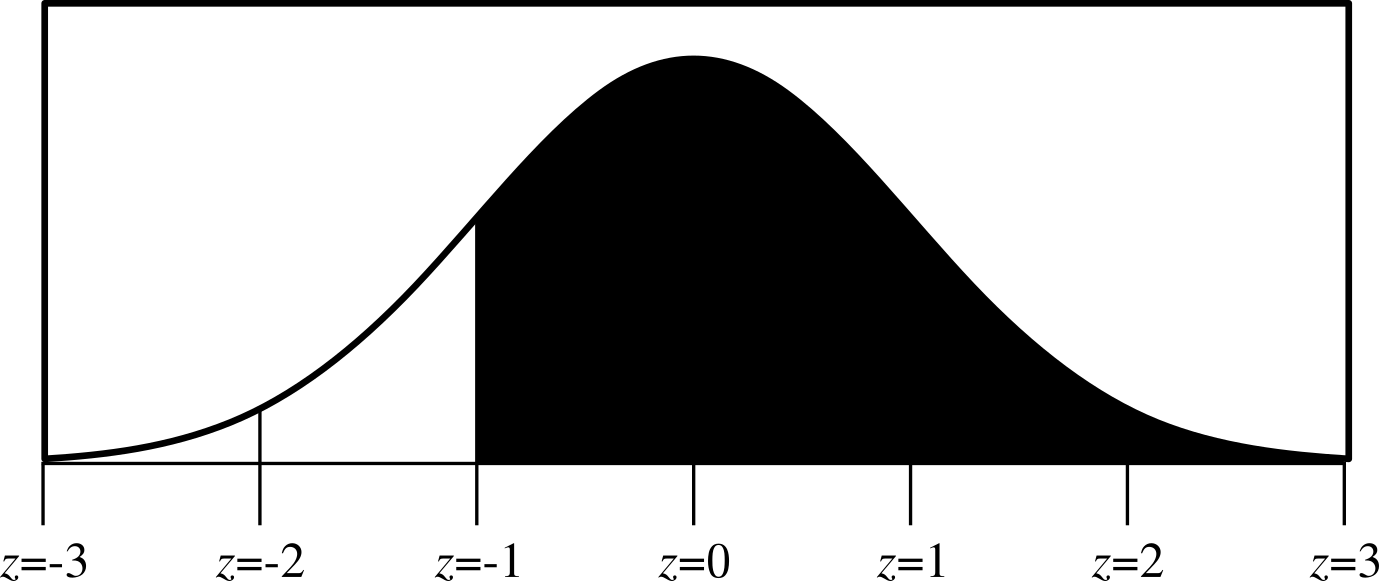
\includegraphics[scale=.5]{n1_3.png}}
\item \adjustbox{valign=t}{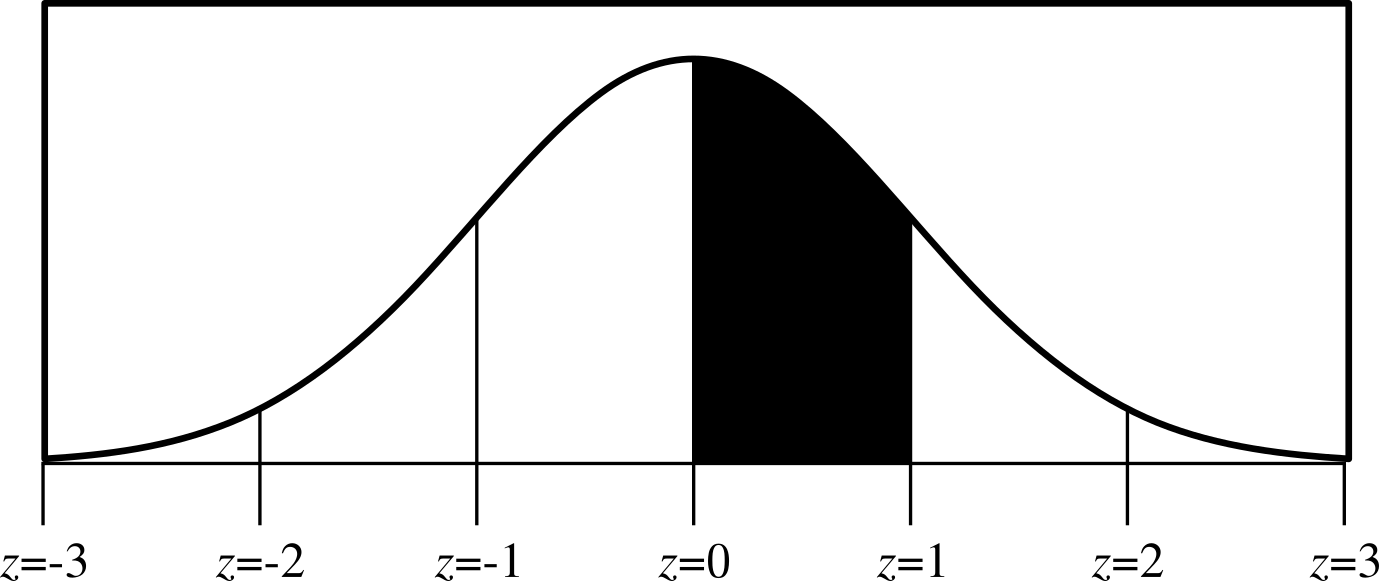
\includegraphics[scale=.5]{0_1.png}}

\columnbreak

\item \adjustbox{valign=t}{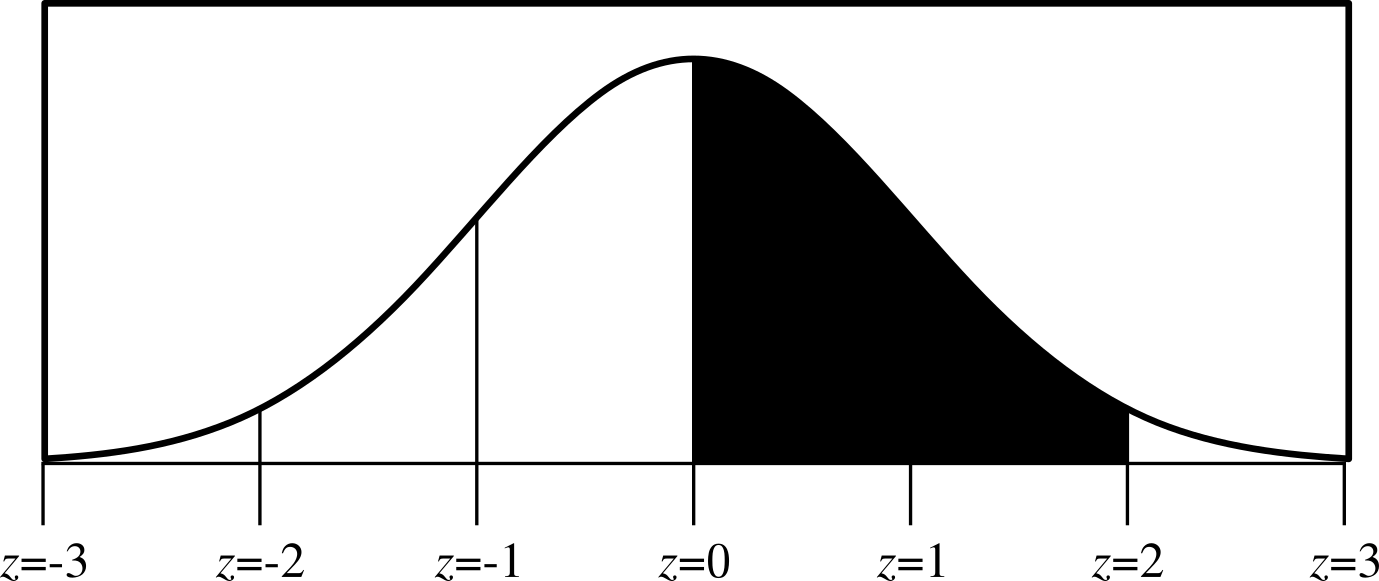
\includegraphics[scale=.5]{0_2.png}}
\item \adjustbox{valign=t}{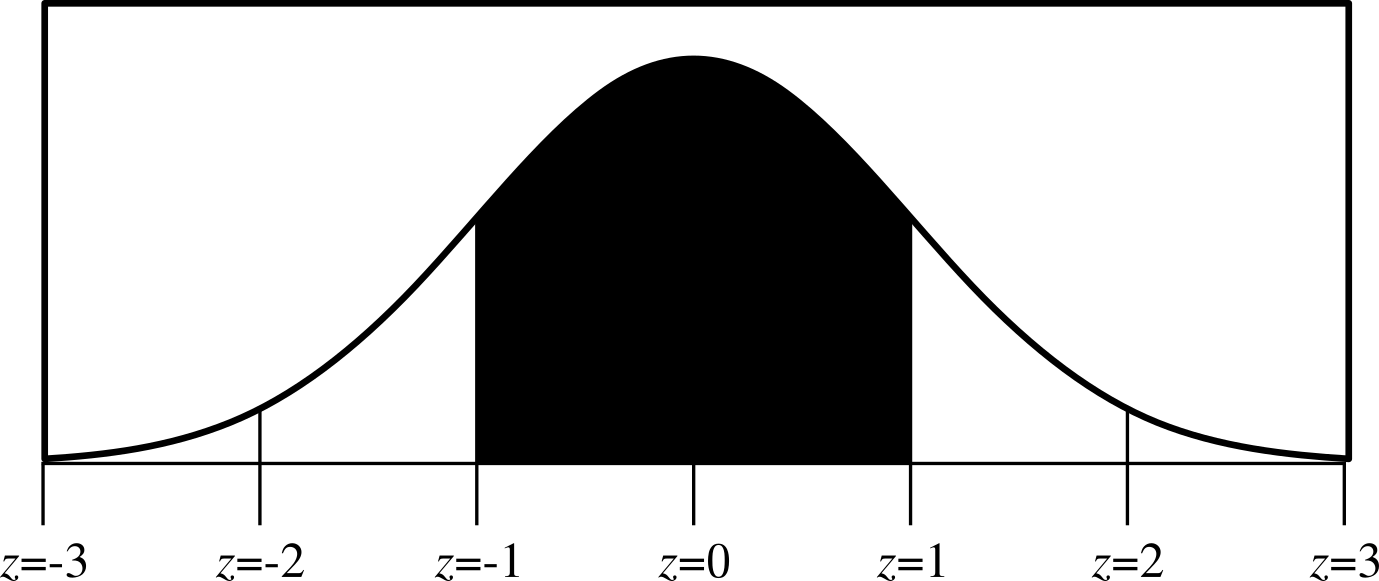
\includegraphics[scale=.5]{n1_1.png}}
\item \adjustbox{valign=t}{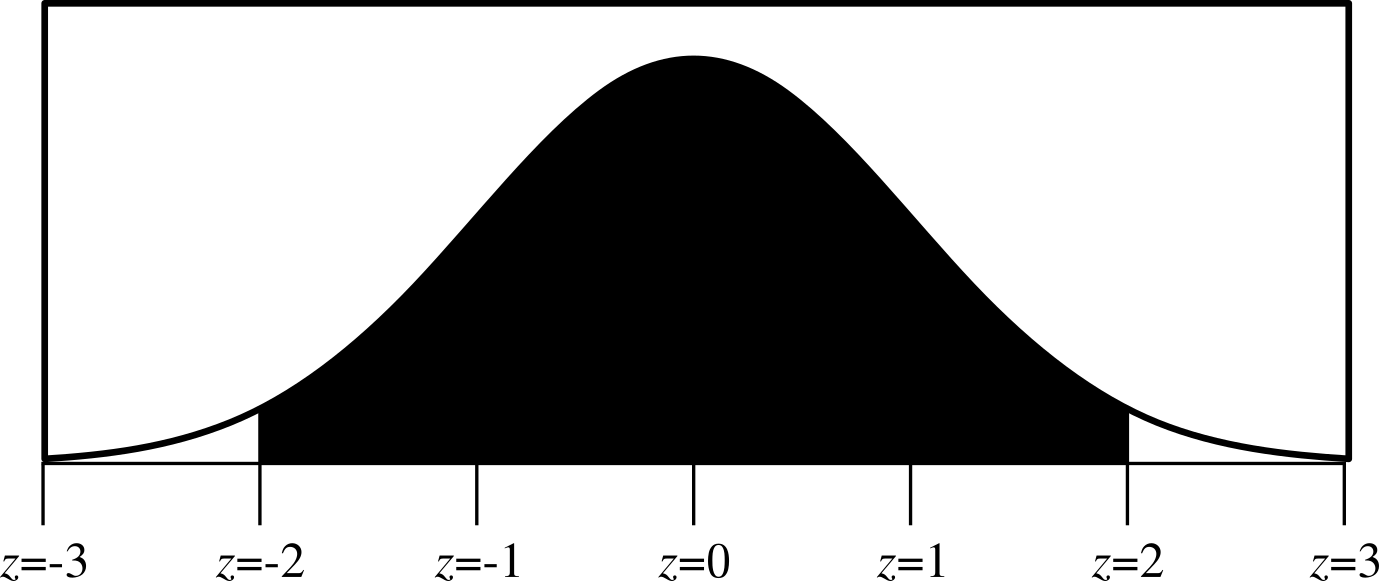
\includegraphics[scale=.5]{n2_2.png}}
\item \adjustbox{valign=t}{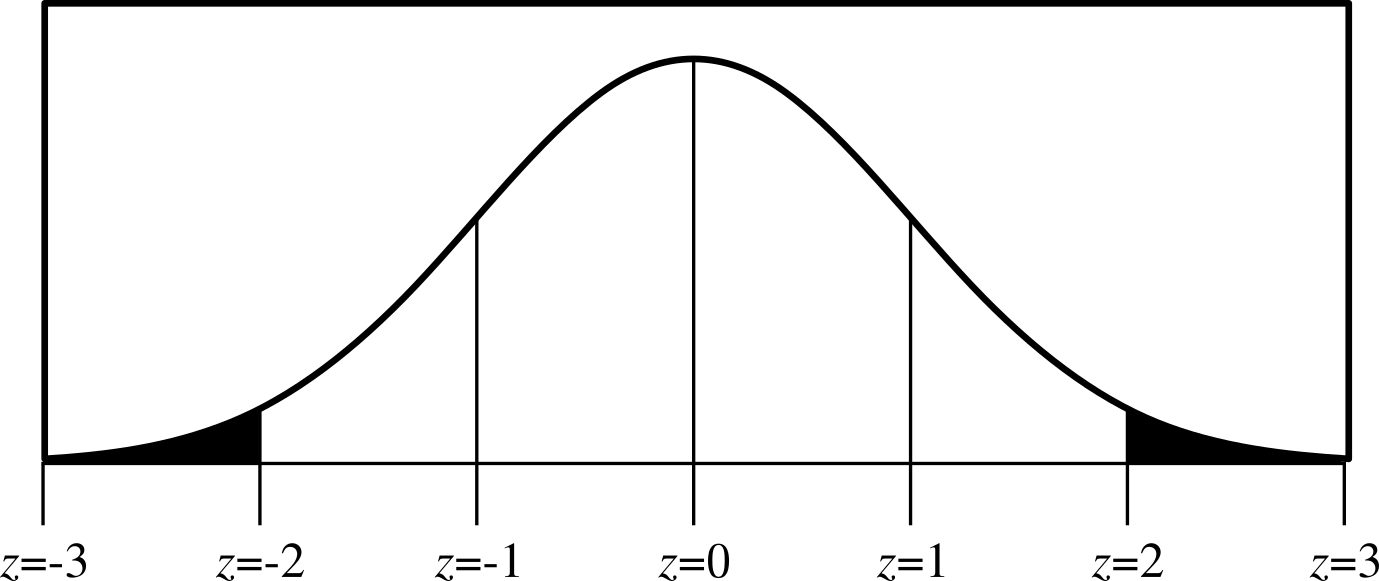
\includegraphics[scale=.5]{n3_n2_and_2_3.png}}
\item \adjustbox{valign=t}{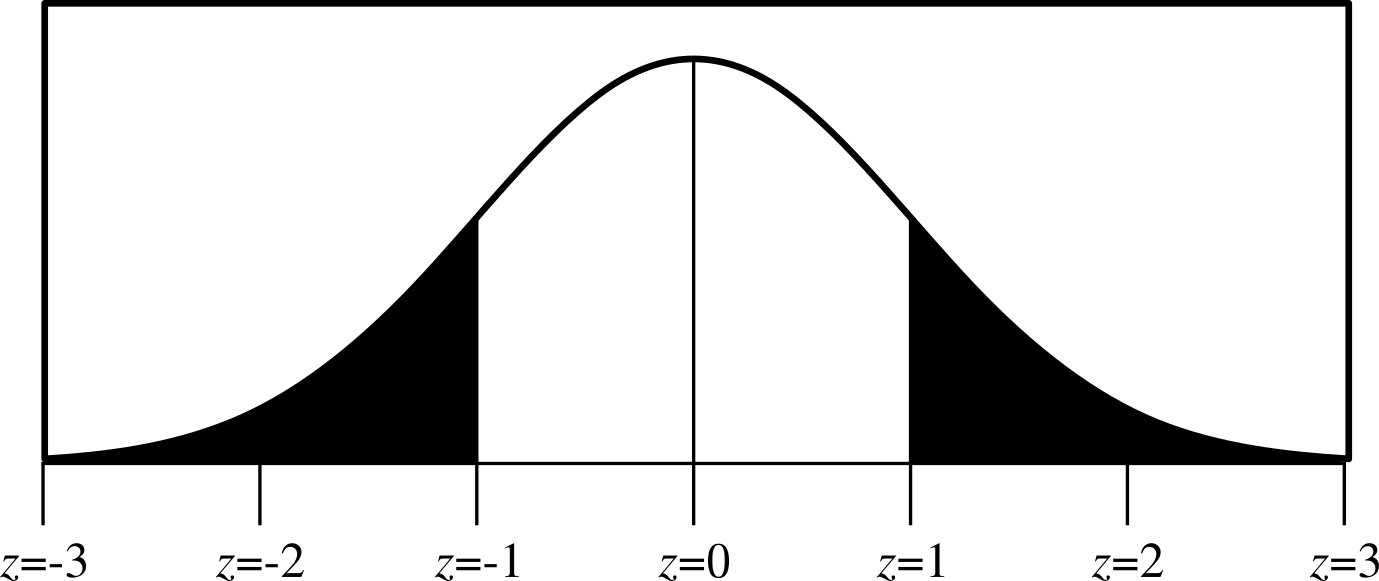
\includegraphics[scale=.5]{n3_n1_and_1_3.png}}

\end{multicols}
\end{enumerate}
\end{enumerate}


\newpage
\subsection*{Central Limit Theorem}
Let the random variable $\bar{X}$ be the mean of a sample of size $n$ taken from a distribution with mean $\mu$ and standard deviation $\sigma$. If $n>30$ then $\bar{X}$ is approximately normally distributed with mean $\mu$ and standard deviation $\frac{\sigma}{\sqrt{n}}$. (If the original distribution is normal, then $n$ can be any number, and the distribution of $\bar{X}$ is exactly normally distributed with mean $\mu$ and standard deviation $\frac{\sigma}{\sqrt{n}}$.)

A typical problem will provide values for $\mu$, $\sigma$, $n$, and boundaries on $\bar{X}$. In these situations, we convert boundaries of $\bar{X}$ into boundaries of $Z$ to calculate the probability.
$$P\Bigl(\bar{x}_1 < \bar{X} < \bar{x}_2\Bigr) ~=~ \,?$$

$$z_1 = \frac{\bar{x}_1-\mu}{\frac{\sigma}{\sqrt{n}}} $$

$$z_2 = \frac{\bar{x}_2-\mu}{\frac{\sigma}{\sqrt{n}}} $$

$$P\Bigl(\bar{x}_1 < \bar{X} < \bar{x}_2\Bigr)~ = ~P\Bigl(z_1 < Z < z_2\Bigr)$$

\subsection*{Normal approximation of binomial distribution}
A binomial distribution can often be approximated by a normal distribution. This de Moivre–Laplace theorem was known before the central limit theorem, but can now be understood as a special case of the central limit theorem.

Let the random variable $X$ represent the number of successes from $n$ trials, each with chance $p$. If $np \ge 5$ and $n(1-p) \ge 5$, then we can approximate the binomial distribution of $X$ as a normal distribution of $Y$ with  $\mu= np$ and $\sigma = \sqrt{np(1-p)}$.

Because a normal distribution is continuous while a binomial distribution is discrete, a continuity correction is made. Some examples:
\begin{align*}
P\Bigl(X < x\Bigr) ~&=~ P\Bigl(Y < x{-}0.5\Bigr) ~=~ P\left(Z < \frac{x-0.5-\mu}{\sigma}\right)\\
P\Bigl(X \le x\Bigr) ~&=~ P\Bigl(Y < x{+}0.5\Bigr) ~=~ P\left(Z < \frac{x+0.5-\mu}{\sigma}\right) \\
P\Bigl(X > x\Bigr) ~&=~ P\Bigl(Y > x{+}0.5\Bigr) ~=~ P\left(Z > \frac{x+0.5-\mu}{\sigma}\right)\\
P\Bigl(X \ge x\Bigr) ~&=~ P\Bigl(Y > x{-}0.5\Bigr) ~=~ P\left(Z > \frac{x-0.5-\mu}{\sigma}\right) \\
P\Bigl(x_1 < X < x_2\Bigr) ~&=~ P\Bigl(x_1+0.5<Y < x_2-0.5\Bigr) ~=~ P\left(\frac{x_1+0.5-\mu}{\sigma}< Z < \frac{x_2-0.5-\mu}{\sigma}\right) \\
P\Bigl(x_1 \le X \le x_2\Bigr) ~&=~ P\Bigl(x_1-0.5 < Y < x_2+0.5\Bigr) ~=~ P\left(\frac{x_1-0.5-\mu}{\sigma}< Z < \frac{x_2+0.5-\mu}{\sigma}\right) \\
P\Bigl(X = x\Bigr) ~&=~ P\Bigl(x-0.5 < Y < x+0.5\Bigr) ~=~ P\left(\frac{x-0.5-\mu}{\sigma}< Z < \frac{x+0.5-\mu}{\sigma}\right) \\
\end{align*}

\newpage
\begin{enumerate}[resume]
\item An individual is measured from a normal distribution with $\mu = 500$ and $\sigma=100$. What is the probability that the individual has a measurement greater than 530?
\vfill
\item If 64 individuals are measured from a continuous distribution with $\mu = 500$ and $\sigma=100$, then what is the probability that their mean is greater than 530?
\vfill
\item If 15 trials each have a 45\% chance of success, then what is the probability of getting exactly 7 successes? Use the normal approximation.
\vfill
\end{enumerate}

\newpage
We have thoroughly practiced finding areas from $z$-scores. We might also want to find $z$-scores from areas. For example, if we wanted to find the value of $z_0$ that satisfies $P(Z<z_0) = 0.86$, we scan the right-columns for $\Phi(z)\approx 0.86$. We find $\Phi(1.08) = 0.8599$.
\begin{center}
\begin{tabular}{|c|c|}\hline
$z$ & $\Phi(z)$ \\ \hline
$\vdots$ & $\vdots$ \\
1.08 & 0.8599 \\
$\vdots$ & $\vdots$ \\ \hline
\end{tabular}
\end{center}
Thus, we estimate $z_0\approx 1.08$. We can also write this as $\Phi^{-1}(0.8599)=1.08$. Here are some formulas for determining $z$ from various areas. These are all derived from equations on page \pageref{hi}.

\begin{align*}
\texttt{Left area} &= A_\text{L}\\
z &= \Phi^{-1}(A_\text{L})\\\\
\texttt{Right area} &= A_\text{R} \\
z &= \Phi^{-1}(1-A_\text{R})\\\\
\texttt{Central area} &= A_\text{C}\\
z &= \Phi^{-1}\left(\frac{A_\text{C}+1}{2}\right)\\\\
\texttt{Two-tailed area} &= A_\text{T} \\
z &= \Phi^{-1}\left(1-\frac{A_\text{T}}{2}\right)
\end{align*}

Remember, these areas also correspond to probabilities. Also, you don't need to memorize these formulas, as you can figure them out by drawing a quick sketch.

\newpage
\begin{enumerate}[resume]
\item \begin{enumerate}
\item Determine $z_0$ such that $\Phi(z_0)=0.0505$. In other words, evaluate $\Phi^{-1}(0.0505)$.
\vfill
\item Determine $z_1$ such that $\Phi(z_1)\approx 0.99$.
\vfill
\item Determine $z_2$ such that $P(Z < z_2) = 55.57\%$
\vfill
\item Determine $z_3$ such that $P(Z > z_3) = 15.87\%$
\vfill
\item Determine $z_4$ such that $P(-z_4 < Z < z_4) = 68.2\%$
\vfill
\item Determine $z_5$ such that $P(|Z| < z_5) = 95\%$
\vfill
\item Determine $z_6$ such that $P(|Z| < z_6) = 90\%$
\vfill
\item Determine $z_7$ such that $P(|Z| > z_7) = 10\%$
\vfill
\end{enumerate}

\newpage
\item If the scores on a test are normally distributed with a mean of 80 and a standard deviation of 10, what score is the 84.1th percentile? (Hint: check out the 68-95-99.7 rule.)
\vfill
\item If the scores on a test are normally distributed with a mean of 80 and a standard deviation of 10, what score is the 97.7th percentile?
\vfill
\item If the scores on a test are normally distributed with a mean of 80 and a standard deviation of 10, what score is the 90th percentile?
\vfill
\item What is the $z$-score such that 68.2\% of the area lies between $-z$ and $z$? (Hint: check out the 68-95-99.7 rule.)
\vfill
\item What is the $z$-score such that 95.4\% of the area lies between $-z$ and $z$?
\vfill
\item What is the $z$-score such that 80\% of the area lies between $-z$ and $z$?
\vfill


\end{enumerate}
\newpage
	\setenumerate[1]{label={\bf A\theenumi: ~}}
	\setenumerate[2]{label={\bf \theenumii: ~}}
\begin{multicols}{2}
\begin{enumerate}
\item \begin{enumerate}
\item $P\bigl(Z < -1.4\bigr) = 0.0808 $\\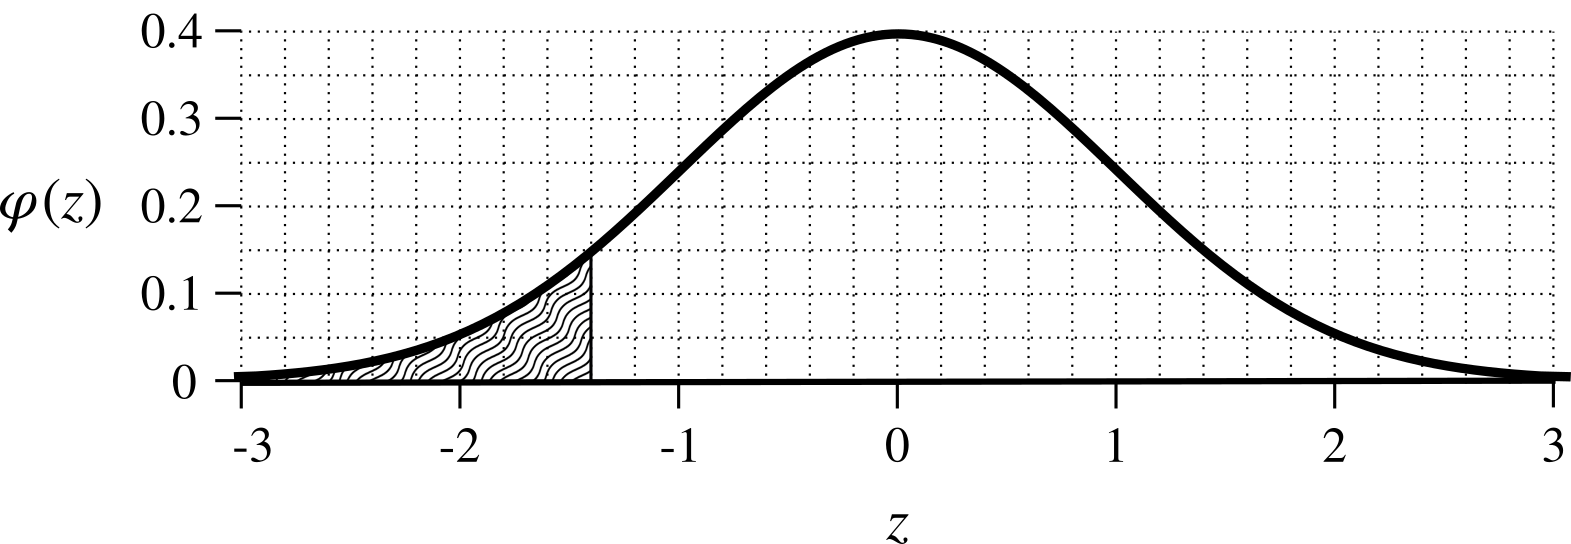
\includegraphics[scale=0.4]{n1p4.png}
\item $P\bigl(Z < 2\bigr) = 0.9772 $\\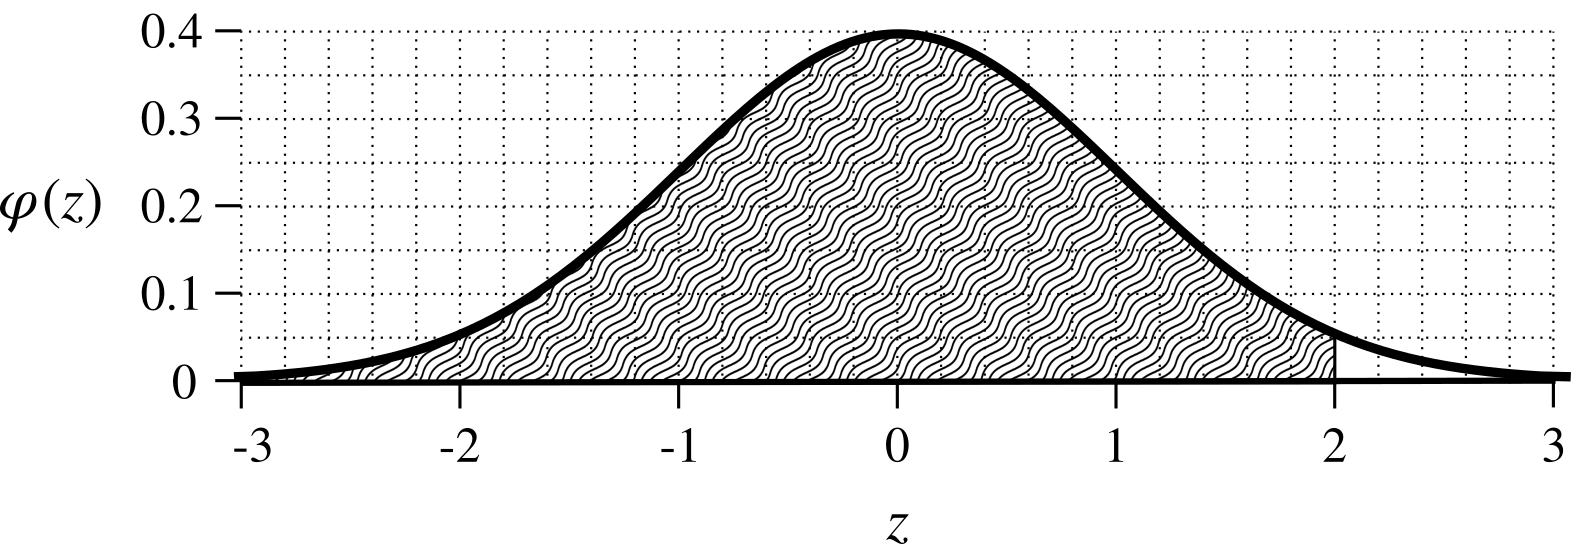
\includegraphics[scale=0.4]{2.png}
\item $P(Z<-0.2) = 0.4207$
\end{enumerate}

\item \begin{enumerate}
\item $P\bigl(Z > 1.6\bigr) = 0.0548 $\\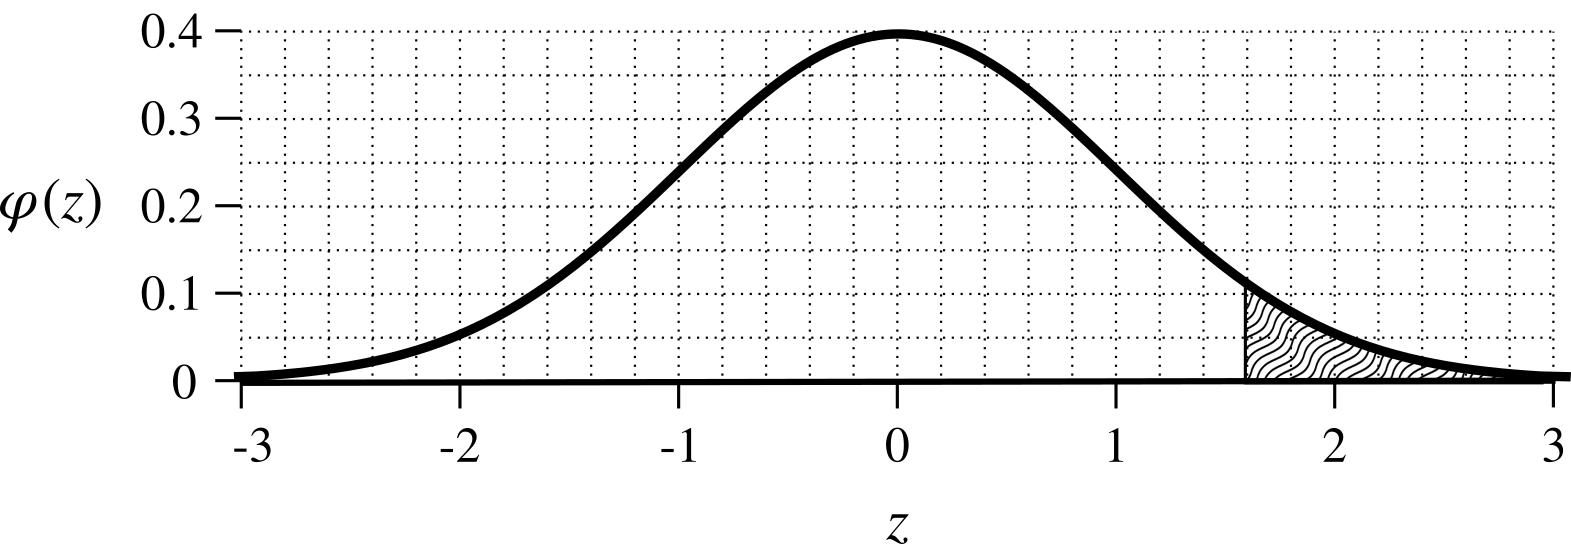
\includegraphics[scale=0.4]{g1p6.png}
\item $P\bigl(0.4 < Z < 0.6\bigr) = 0.0703 $\\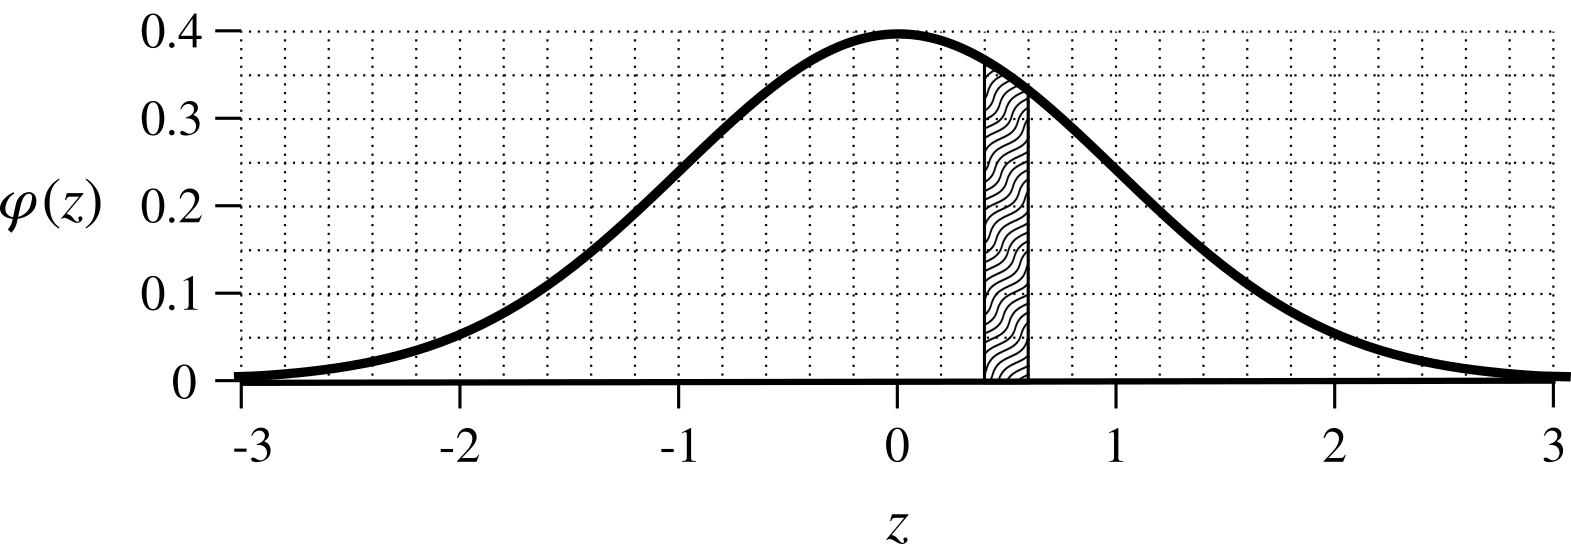
\includegraphics[scale=0.4]{bp4p6.png}
\item $P\bigl(1 < Z < 2\bigr) = 0.1359 $\\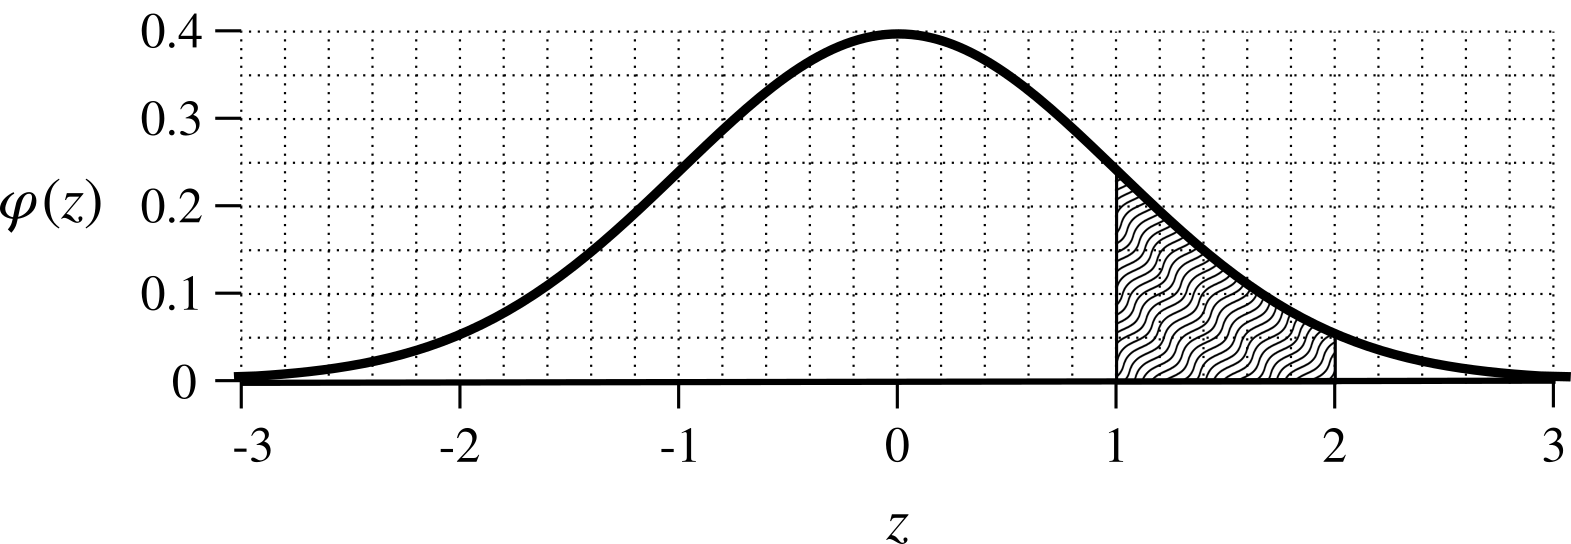
\includegraphics[scale=0.4]{b1a2.png}
\item $P\bigl(|Z| < 0.4\bigr) = 0.3108 $\\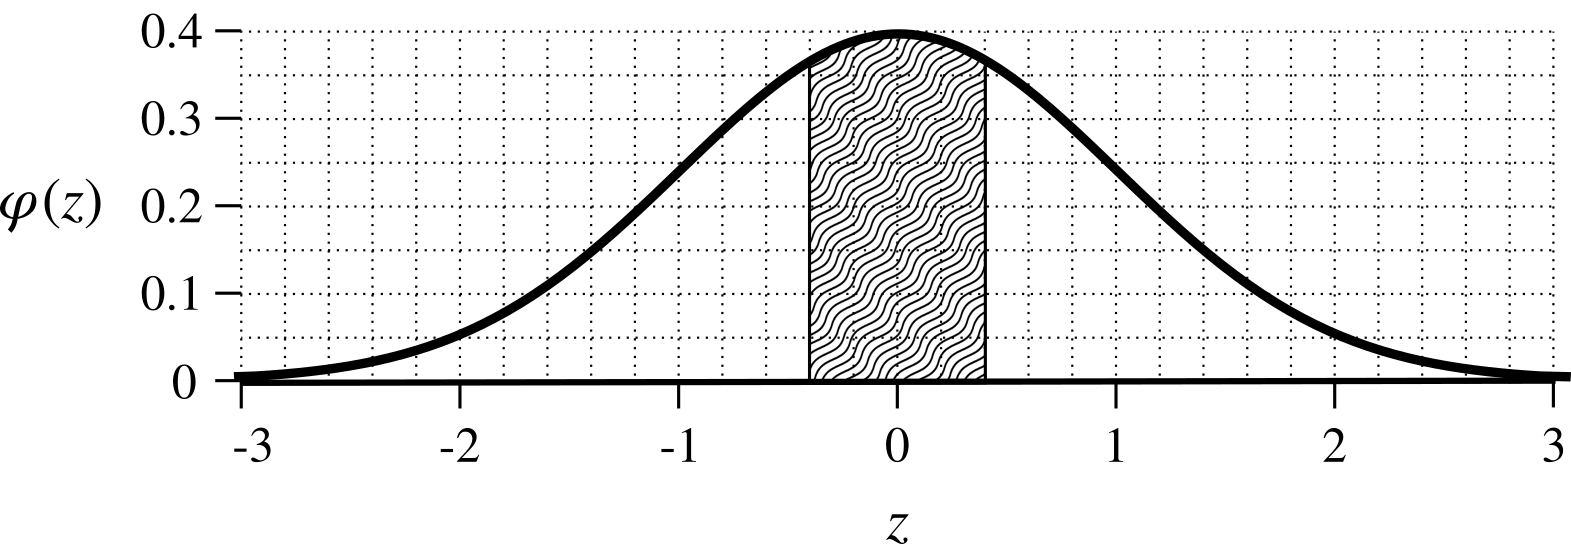
\includegraphics[scale=0.4]{alp4.png}
\item $P\bigl(|Z| > 0.4\bigr) = 0.6892 $\\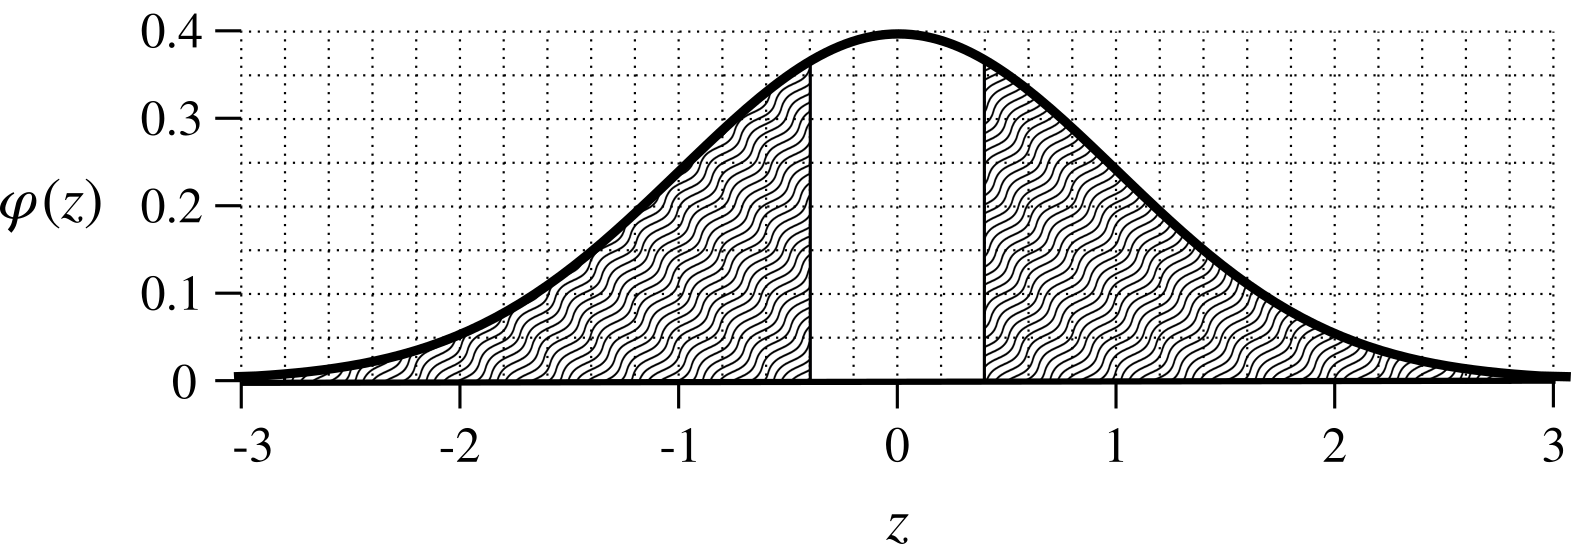
\includegraphics[scale=0.4]{agp4.png}
\end{enumerate}
\columnbreak
\item \begin{enumerate}
\item $P(Z<-1)=0.159$
\item $P(Z<0) = 0.5$
\item $P(Z<1) = 0.841$
\item $P(-1<Z) = 0.841$
\item $P(0<Z<1) = 0.341$
\item $P(0<Z<2) = 0.477$
\item $P(|Z|<1) = 0.682$
\item $P(|Z|<2) = 0.954$
\item $P(|Z|>2) = 0.046$
\item $P(|Z|>1) = 0.318$
\end{enumerate}

\item $0.3821$
\item $0.0082$
\item $0.2031$

\item \begin{enumerate}
\item $z_0 = -1.64$
\item $z_1 = 2.33$
\item $z_2 = 0.14$
\item $z_3 = 1$
\item $z_4 = 1$
\item $z_5 = 1.96$
\item $z_6 = 1.64$
\item $z_7 = 1.64$
\end{enumerate}

\item 90.0
\item 100.0
\item $z = \Phi^{-1}(0.9) = 1.2815
\\(1.2815)(10)+80 \approx \fbox{92.8}$
\item $z=1$
\item $z=2$
\item $z = \Phi^{-1}\Bigl(\frac{0.8+1}{2}\Bigr)=\Phi^{-1}(0.9)=1.282$

\end{enumerate}
\end{multicols}

\end{document}
